\hypertarget{sec-optimization}{%
\chapter{Hyperparameter Optimization}\label{sec-optimization}}

\vspace{-15mm}\addtocontents{toc}{\textit{Marc Becker, Lennart Schneider and Sebastian Fischer}}

\textbf{Marc Becker} \newline  \emph{Ludwig-Maximilians-Universität
München, and Munich Center for Machine Learning (MCML)}

\textbf{Lennart Schneider} \newline 
\emph{Ludwig-Maximilians-Universität München, and Munich Center for
Machine Learning (MCML)}

\textbf{Sebastian Fischer} \newline 
\emph{Ludwig-Maximilians-Universität München, and Munich Center for
Machine Learning (MCML)} \newline \newline 

Machine learning algorithms usually include parameters\index{parameters}
and
hyperparameters\index{hyperparameters}{\marginnote{\begin{footnotesize}Hyperparameters\end{footnotesize}}}.
Parameters are the model
coefficients\index{model coefficients|see{parameters}} or weights or
other information that are determined by the learning algorithm based on
the training data. In contrast, hyperparameters, are configured by the
user and determine how the model will fit its parameters, i.e., how the
model is built. Examples include setting the number of trees in a random
forest, penalty settings in support vector machines, or the learning
rate in a neural network.

The goal of hyperparameter
optimization\index{HPO}{\marginnote{\begin{footnotesize}Hyperparameter
Optimization\end{footnotesize}}}\index{hyperparameter optimization|see{HPO}}
(HPO) or model tuning\index{tuning} is to find the optimal configuration
of hyperparameters of a machine learning algorithm for a given task.
There is no closed-form mathematical representation (nor analytic
gradient information) for model-agnostic HPO. Instead, we follow a black
box optimization\index{black box optimization} approach: a machine
learning algorithm is configured with values chosen for one or more
hyperparameters, this algorithm is then evaluated (using a resampling
method) and its performance is measured. This process is repeated with
multiple configurations and finally, the configuration with the best
performance is selected (Figure~\ref{fig-optimization-loop-basic}). HPO
closely relates to model evaluation\index{model evaluation}
(Chapter~\ref{sec-performance}) as the objective is to find a
hyperparameter configuration that optimizes the generalization
performance. Broadly speaking, we could think of finding the optimal
model configuration in the same way as selecting a model from a
benchmark experiment, where in this case each model in the experiment is
the same algorithm but with different hyperparameter configurations. For
example, we could benchmark three support vector
machines\index{support vector machine} (SVMs) with three different
\texttt{cost} values. However, human trial-and-error is time-consuming,
subjective and often biased, error-prone, and computationally
inefficient. Instead, many sophisticated hyperparameter optimization
methods (or `tuners\index{tuners}', see Section~\ref{sec-tuner}) have
been developed over the past few decades for robust and efficient HPO.
Besides simple approaches such as a random search\index{random search}
or grid search\index{grid search}, most hyperparameter optimization
methods employ iterative techniques that propose different
configurations over time, often exhibiting adaptive behavior guided
towards potentially optimal hyperparameter configurations. These methods
continually propose new configurations until a termination criterion is
met, at which point the best configuration so far is returned
(Figure~\ref{fig-optimization-loop-basic}). For more general details on
HPO and more theoretical background, we recommend Bischl et al. (2023)
and Feurer and Hutter (2019).

\begin{figure}

{\centering 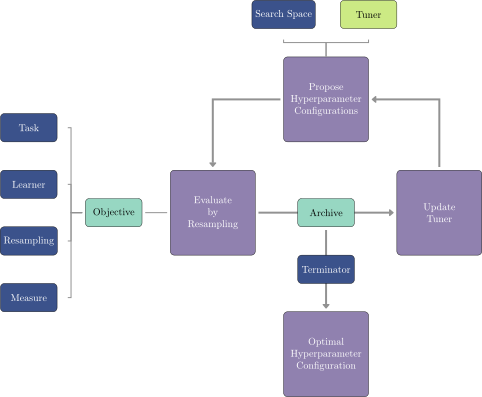
\includegraphics[width=0.8\textwidth]{chapters/chapter4/Figures/mlr3book_figures-9.png}

}

\caption{\label{fig-optimization-loop-basic}Representation of the
hyperparameter optimization loop in mlr3tuning. Blue - Hyperparameter
optimization loop. Purple - Objects of the tuning instance supplied by
the user. Blue-Green - Internally created objects of the tuning
instance. Green - Optimization Algorithm.}

\end{figure}

\hypertarget{sec-model-tuning}{%
\section{Model Tuning}\label{sec-model-tuning}}

\href{https://mlr3tuning.mlr-org.com}{\texttt{mlr3tuning}}\index{\texttt{mlr3tuning}}
is the hyperparameter optimization package of the \texttt{mlr3}
ecosystem. At the heart of the package are the R6 classes

\begin{itemize}
\tightlist
\item
  \href{https://mlr3tuning.mlr-org.com/reference/TuningInstanceSingleCrit.html}{\texttt{TuningInstanceSingleCrit}},
  a tuning `instance' that describes the optimization problem and store
  the results; and
\item
  \href{https://mlr3tuning.mlr-org.com/reference/Tuner.html}{\texttt{Tuner}}
  which is used to configure and run optimization algorithms.
\end{itemize}

In this section, we will cover these classes as well as other supporting
functions and classes. Throughout this section, we will look at
optimizing an SVM classifier\index{support vector machine} from
\href{https://cran.r-project.org/package=e1071}{\texttt{e1071}} on
\texttt{tsk("sonar")} as a running example.

\hypertarget{sec-learner-search-space}{%
\subsection{Learner and Search Space}\label{sec-learner-search-space}}

The tuning process begins by deciding which hyperparameters to tune and
what range to tune them over. The first place to start is therefore
picking a learner and looking at the possible hyperparameters to tune
with \texttt{\$param\_set}:

\begin{Shaded}
\begin{Highlighting}[]
\FunctionTok{as.data.table}\NormalTok{(}\FunctionTok{lrn}\NormalTok{(}\StringTok{"classif.svm"}\NormalTok{)}\SpecialCharTok{$}\NormalTok{param\_set)[,}
\NormalTok{  .(id, class, lower, upper, nlevels)]}
\end{Highlighting}
\end{Shaded}

\begin{verbatim}
               id    class lower upper nlevels
 1:     cachesize ParamDbl  -Inf   Inf     Inf
 2: class.weights ParamUty    NA    NA     Inf
 3:         coef0 ParamDbl  -Inf   Inf     Inf
 4:          cost ParamDbl     0   Inf     Inf
 5:         cross ParamInt     0   Inf     Inf
---                                           
12:            nu ParamDbl  -Inf   Inf     Inf
13:         scale ParamUty    NA    NA     Inf
14:     shrinking ParamLgl    NA    NA       2
15:     tolerance ParamDbl     0   Inf     Inf
16:          type ParamFct    NA    NA       2
\end{verbatim}

Given infinite resources, we could tune all hyperparameters jointly, but
in reality that is not possible (or maybe necessary), so usually only a
subset of hyperparameters can be tuned. This subset of possible
hyperparameter values to tune over is referred to as the search
space\index{search space}{\marginnote{\begin{footnotesize}Search
Space\end{footnotesize}}} or tuning
space\index{tuning space|see{search space}}. In this example we will
tune the numeric regularization and kernel width hyperparameters,
\texttt{cost} and \texttt{gamma}; see the help page for
\href{https://www.rdocumentation.org/packages/e1071/topics/svm}{\texttt{svm()}}
for details. In practice, search spaces are usually more complex and can
require expert knowledge to define them.
Section~\ref{sec-defining-search-spaces} provides more detailed insight
into the creation of tuning spaces, including using
\href{https://mlr3tuningspaces.mlr-org.com}{\texttt{mlr3tuningspaces}}\index{\texttt{mlr3tuningspaces}}
to load predefined search spaces.

\begin{tcolorbox}[enhanced jigsaw, opacitybacktitle=0.6, rightrule=.15mm, opacityback=0, arc=.35mm, breakable, titlerule=0mm, colframe=quarto-callout-tip-color-frame, coltitle=black, bottomrule=.15mm, toprule=.15mm, colback=white, colbacktitle=quarto-callout-tip-color!10!white, bottomtitle=1mm, toptitle=1mm, title=\textcolor{quarto-callout-tip-color}{\faLightbulb}\hspace{0.5em}{Untunable Hyperparameters}, leftrule=.75mm, left=2mm]

In rare cases, parameter sets may include hyperparameters that should
not be tuned. These will usually be `technical' (or `control')
parameters that \emph{provide information} about how the model is being
fit but do not control the training process itself, for example, the
\texttt{verbose} hyperparameter in \texttt{lrn("classif.ranger")}
controls how much information is displayed to the user during training.

\end{tcolorbox}

For numeric hyperparameters (we will explore others later) one must
specify the bounds to tune over. We do this by constructing a learner
and using
\href{https://paradox.mlr-org.com/reference/to_tune.html}{\texttt{to\_tune()}}
to set the lower and upper limits for the parameters we want to tune.
This function allows us to \emph{mark} the hyperparameter as requiring
tuning in the specified range.

\begin{Shaded}
\begin{Highlighting}[]
\NormalTok{learner }\OtherTok{=} \FunctionTok{lrn}\NormalTok{(}\StringTok{"classif.svm"}\NormalTok{,}
  \AttributeTok{type  =} \StringTok{"C{-}classification"}\NormalTok{,}
  \AttributeTok{kernel =} \StringTok{"radial"}\NormalTok{,}
  \AttributeTok{cost  =} \FunctionTok{to\_tune}\NormalTok{(}\FloatTok{1e{-}1}\NormalTok{, }\FloatTok{1e5}\NormalTok{),}
  \AttributeTok{gamma =} \FunctionTok{to\_tune}\NormalTok{(}\FloatTok{1e{-}1}\NormalTok{, }\DecValTok{1}\NormalTok{)}
\NormalTok{)}
\NormalTok{learner}
\end{Highlighting}
\end{Shaded}

\begin{verbatim}
<LearnerClassifSVM:classif.svm>
* Model: -
* Parameters: type=C-classification, kernel=radial,
  cost=<RangeTuneToken>, gamma=<RangeTuneToken>
* Packages: mlr3, mlr3learners, e1071
* Predict Types:  [response], prob
* Feature Types: logical, integer, numeric
* Properties: multiclass, twoclass
\end{verbatim}

Here we have constructed a classification SVM,
\texttt{lrn("classif.svm")}, selected the type of model as
\texttt{"C-classification"}, set the kernel to \texttt{"radial"}, and
specified that we plan to tune the \texttt{cost} and \texttt{gamma}
parameters over the range \([0.1, 10^5]\) and \([0.1, 1]\) respectively
(though these are usually tuned on a log scale, see
Section~\ref{sec-logarithmic-transformations}). Note that calling
\texttt{\$train()} on a learner with a tune token (e.g.,
\texttt{cost=\textless{}RangeTuneToken\textgreater{}}) will throw an
error.

Now we have decided which hyperparameters to tune, we specify when to
stop the tuning process.

\hypertarget{sec-terminator}{%
\subsection{Terminator}\label{sec-terminator}}

\texttt{mlr3tuning} includes many methods to specify when to terminate
an algorithm (Table~\ref{tbl-terms}), which are implemented in
\href{https://bbotk.mlr-org.com/reference/Terminator.html}{\texttt{Terminator}}\index{\texttt{Terminator}}{\marginnote{\begin{footnotesize}\texttt{Terminator}\end{footnotesize}}}
classes. Terminators are stored in the
\href{https://bbotk.mlr-org.com/reference/mlr_terminators.html}{\texttt{mlr\_terminators}}
dictionary and are constructed with the sugar function
\href{https://bbotk.mlr-org.com/reference/trm.html}{\texttt{trm()}}\index{\texttt{trm()}}{\marginnote{\begin{footnotesize}\texttt{trm()}\end{footnotesize}}}.

\hypertarget{tbl-terms}{}
\begin{longtable}[]{@{}
  >{\raggedright\arraybackslash}p{(\columnwidth - 2\tabcolsep) * \real{0.2396}}
  >{\raggedright\arraybackslash}p{(\columnwidth - 2\tabcolsep) * \real{0.7604}}@{}}
\caption{\label{tbl-terms}Terminators available in \texttt{mlr3tuning}
at the time of publication, their function call and default parameters.
A complete and up-to-date list can be found at
\url{https://mlr-org.com/terminators.html}.}\tabularnewline
\toprule\noalign{}
\begin{minipage}[b]{\linewidth}\raggedright
Terminator
\end{minipage} & \begin{minipage}[b]{\linewidth}\raggedright
Function call and default parameters
\end{minipage} \\
\midrule\noalign{}
\endfirsthead
\toprule\noalign{}
\begin{minipage}[b]{\linewidth}\raggedright
Terminator
\end{minipage} & \begin{minipage}[b]{\linewidth}\raggedright
Function call and default parameters
\end{minipage} \\
\midrule\noalign{}
\endhead
\bottomrule\noalign{}
\endlastfoot
Clock Time & \texttt{trm("clock\_time")} \\
Combo & \texttt{trm("combo",\ any\ =\ TRUE)} \\
None & \texttt{trm("none")} \\
Number of Evaluations &
\texttt{trm("evals",\ n\_evals\ =\ 100,\ k\ =\ 0)} \\
Performance Level & \texttt{trm("perf\_reached",\ level\ =\ 0.1)} \\
Run Time & \texttt{trm("run\_time",\ secs\ =\ 30)} \\
Stagnation &
\texttt{trm("stagnation",\ iters\ =\ 10,\ threshold\ =\ 0)} \\
\end{longtable}

The most commonly used terminators are those that stop the tuning after
a certain time (\texttt{trm("run\_time")}) or a given number of
evaluations (\texttt{trm("evals")}). Choosing a runtime is often based
on practical considerations and intuition. Using a time limit can be
important on compute clusters where a maximum runtime for a compute job
may need to be specified. \texttt{trm("perf\_reached")} stops the tuning
when a specified performance level is reached, which can be helpful if a
certain performance is seen as sufficient for the practical use of the
model, however, if this is set too optimistically the tuning may never
terminate. \texttt{trm("stagnation")} stops when no progress greater
than the \texttt{threshold} has been made for a set number of
\texttt{iterations}. The threshold can be difficult to select as the
optimization could stop too soon for complex search spaces despite room
for (possibly significant) improvement. \texttt{trm("none")} is used for
tuners that control termination themselves and so this terminator does
nothing. Finally, any of these terminators can be freely combined by
using \texttt{trm("combo")}, which can be used to specify if HPO
finishes when any (\texttt{any\ =\ TRUE}) terminator is triggered or
when all (\texttt{any\ =\ FALSE}) are triggered.

\hypertarget{sec-tuning-instance}{%
\subsection{\texorpdfstring{Tuning Instance with
\texttt{ti}}{Tuning Instance with ti}}\label{sec-tuning-instance}}

The tuning instance collects the tuner-agnostic information required to
optimize a model, i.e., all information about the tuning process, except
for the tuning algorithm itself. This includes the task to tune over,
the learner to tune, the resampling method and measure used to
analytically compare hyperparameter optimization configurations, and the
terminator to determine when the measure has been optimized `enough'.
This implicitly defines a ``black box'' objective function, mapping
hyperparameter configurations to (stochastic) performance values, to be
optimized. This concept will be revisited in
Chapter~\ref{sec-optimization-advanced}.

A tuning instance\index{tuning instance} can be constructed explicitly
with the
\href{https://mlr3tuning.mlr-org.com/reference/ti.html}{\texttt{ti()}}
function, or we can tune a learner with the
\href{https://mlr3tuning.mlr-org.com/reference/tune.html}{\texttt{tune()}}
function, which implicitly creates a tuning instance, as shown in
Section~\ref{sec-autotuner}. We cover the \texttt{ti()} approach first
as this allows finer control of tuning and a more nuanced discussion
about the design and use of \texttt{mlr3tuning}.

Continuing our example, we will construct a
single-objective\index{single-objective} tuning problem (i.e., tuning
over \emph{one} measure) by using the \texttt{ti()} function to create a
\href{https://mlr3tuning.mlr-org.com/reference/TuningInstanceSingleCrit.html}{\texttt{TuningInstanceSingleCrit}},
we will return to multi-objective tuning\index{multi-objective tuning}
in Section~\ref{sec-multi-metrics-tuning}.

For this example, we will use three-fold CV and optimize the
classification error measure. Note that in the next section, we will
continue our example with a grid search tuner, so we select
\texttt{trm("none")} below as we will want to iterate over the full grid
without stopping too soon.

\begin{Shaded}
\begin{Highlighting}[]
\NormalTok{tsk\_sonar }\OtherTok{=} \FunctionTok{tsk}\NormalTok{(}\StringTok{"sonar"}\NormalTok{)}

\NormalTok{learner }\OtherTok{=} \FunctionTok{lrn}\NormalTok{(}\StringTok{"classif.svm"}\NormalTok{,}
  \AttributeTok{cost  =} \FunctionTok{to\_tune}\NormalTok{(}\FloatTok{1e{-}1}\NormalTok{, }\FloatTok{1e5}\NormalTok{),}
  \AttributeTok{gamma =} \FunctionTok{to\_tune}\NormalTok{(}\FloatTok{1e{-}1}\NormalTok{, }\DecValTok{1}\NormalTok{),}
  \AttributeTok{kernel =} \StringTok{"radial"}\NormalTok{,}
  \AttributeTok{type =} \StringTok{"C{-}classification"}
\NormalTok{)}

\NormalTok{instance }\OtherTok{=} \FunctionTok{ti}\NormalTok{(}
  \AttributeTok{task =}\NormalTok{ tsk\_sonar,}
  \AttributeTok{learner =}\NormalTok{ learner,}
  \AttributeTok{resampling =} \FunctionTok{rsmp}\NormalTok{(}\StringTok{"cv"}\NormalTok{, }\AttributeTok{folds =} \DecValTok{3}\NormalTok{),}
  \AttributeTok{measures =} \FunctionTok{msr}\NormalTok{(}\StringTok{"classif.ce"}\NormalTok{),}
  \AttributeTok{terminator =} \FunctionTok{trm}\NormalTok{(}\StringTok{"none"}\NormalTok{)}
\NormalTok{)}

\NormalTok{instance}
\end{Highlighting}
\end{Shaded}

\begin{verbatim}
<TuningInstanceSingleCrit>
* State:  Not optimized
* Objective: <ObjectiveTuning:classif.svm_on_sonar>
* Search Space:
      id    class lower upper nlevels
1:  cost ParamDbl   0.1 1e+05     Inf
2: gamma ParamDbl   0.1 1e+00     Inf
* Terminator: <TerminatorNone>
\end{verbatim}

\hypertarget{sec-tuner}{%
\subsection{Tuner}\label{sec-tuner}}

With all the pieces of our tuning problem assembled, we can now decide
\emph{how} to tune our model. There are multiple
\href{https://mlr3tuning.mlr-org.com/reference/Tuner.html}{\texttt{Tuner}}\index{\texttt{Tuner}}{\marginnote{\begin{footnotesize}\texttt{Tuner}\end{footnotesize}}}
classes in \texttt{mlr3tuning}, which implement different HPO (or more
generally speaking black box optimization\index{black box optimization})
algorithms (Table~\ref{tbl-tuners}).

\hypertarget{tbl-tuners}{}
\begin{longtable}[]{@{}
  >{\raggedright\arraybackslash}p{(\columnwidth - 4\tabcolsep) * \real{0.4125}}
  >{\raggedright\arraybackslash}p{(\columnwidth - 4\tabcolsep) * \real{0.3000}}
  >{\raggedright\arraybackslash}p{(\columnwidth - 4\tabcolsep) * \real{0.2875}}@{}}
\caption{\label{tbl-tuners}Tuning algorithms available in
\texttt{mlr3tuning}, their function call and the package in which the
algorithm is implemented. A complete and up-to-date list can be found at
\url{https://mlr-org.com/tuners.html}.}\tabularnewline
\toprule\noalign{}
\begin{minipage}[b]{\linewidth}\raggedright
Tuner
\end{minipage} & \begin{minipage}[b]{\linewidth}\raggedright
Function call
\end{minipage} & \begin{minipage}[b]{\linewidth}\raggedright
Package
\end{minipage} \\
\midrule\noalign{}
\endfirsthead
\toprule\noalign{}
\begin{minipage}[b]{\linewidth}\raggedright
Tuner
\end{minipage} & \begin{minipage}[b]{\linewidth}\raggedright
Function call
\end{minipage} & \begin{minipage}[b]{\linewidth}\raggedright
Package
\end{minipage} \\
\midrule\noalign{}
\endhead
\bottomrule\noalign{}
\endlastfoot
Random Search & \texttt{tnr("random\_search")} &
\href{https://mlr3tuning.mlr-org.com}{\texttt{mlr3tuning}}\index{\texttt{mlr3tuning}} \\
Grid Search & \texttt{tnr("grid\_search")} &
\href{https://mlr3tuning.mlr-org.com}{\texttt{mlr3tuning}}\index{\texttt{mlr3tuning}} \\
Bayesian Optimization & \texttt{tnr("mbo")} &
\href{https://mlr3mbo.mlr-org.com}{\texttt{mlr3mbo}}\index{\texttt{mlr3mbo}} \\
CMA-ES & \texttt{tnr("cmaes")} &
\href{https://cran.r-project.org/package=adagio}{\texttt{adagio}} \\
Iterated Racing & \texttt{tnr("irace")} &
\href{https://cran.r-project.org/package=irace}{\texttt{irace}} \\
Hyperband & \texttt{tnr("hyperband")} &
\href{https://mlr3hyperband.mlr-org.com}{\texttt{mlr3hyperband}}\index{\texttt{mlr3hyperband}} \\
Generalized Simulated Annealing & \texttt{tnr("gensa")} &
\href{https://cran.r-project.org/package=GenSA}{\texttt{GenSA}} \\
Nonlinear Optimization & \texttt{tnr("nloptr")} &
\href{https://cran.r-project.org/package=nloptr}{\texttt{nloptr}} \\
\end{longtable}

\hypertarget{search-strategies}{%
\subsubsection*{Search strategies}\label{search-strategies}}

Grid search and random search (Bergstra and Bengio 2012) are the most
basic algorithms and are often selected first in initial experiments.
The idea of grid search is to exhaustively evaluate every possible
combination of given hyperparameter values. Categorical hyperparameters
are usually evaluated over all possible values they can take. Numeric
and integer hyperparameter values are then spaced equidistantly in their
box constraints (upper and lower bounds) according to a given
resolution, which is the number of distinct values to try per
hyperparameter. Random search involves randomly selecting values for
each hyperparameter independently from a pre-specified distribution,
usually uniform. Both methods are non-adaptive, which means each
proposed configuration ignores the performance of previous
configurations. Due to their simplicity, both grid search and random
search can handle mixed search spaces (i.e., hyperparameters can be
numeric, integer, or categorical) as well as hierarchical search spaces
(Section~\ref{sec-defining-search-spaces}).

\hypertarget{adaptive-algorithms}{%
\subsubsection*{Adaptive algorithms}\label{adaptive-algorithms}}

Adaptive algorithms learn from previously evaluated configurations to
find good configurations quickly, examples in
\href{https://mlr3.mlr-org.com}{\texttt{mlr3}}\index{\texttt{mlr3}}
include Bayesian optimization (also called model-based optimization),
Covariance Matrix Adaptation Evolution Strategy (CMA-ES), Iterated
Racing\index{iterated racing}, and Hyperband.

Bayesian optimization\index{Bayesian optimization} (e.g., Snoek,
Larochelle, and Adams 2012) describes a family of iterative optimization
algorithms that use a surrogate model to approximate the unknown
function that is to be optimized -- in HPO this would be the mapping
from a hyperparameter configuration to the estimated generalization
performance. If a suitable surrogate model is chosen, e.g.~a random
forest, Bayesian optimization can be quite flexible and even handle
mixed and hierarchical search spaces. Bayesian optimization is discussed
in full detail in Section~\ref{sec-bayesian-optimization}.

CMA-ES\index{CMA-ES} (Hansen and Auger 2011) is an evolutionary
strategy\index{evolutionary strategies} that maintains a probability
distribution over candidate points, with the distribution represented by
a mean vector and covariance matrix. A new set of candidate points is
generated by sampling from this distribution, with the probability of
each candidate being proportional to its performance. The covariance
matrix is adapted over time to reflect the performance landscape.
Further evolutionary strategies are available in \texttt{mlr3} via the
\href{https://cran.r-project.org/package=miesmuschel}{\texttt{miesmuschel}}
package, however, these will not be covered in this book.

Racing algorithms work by iteratively discarding configurations that
show poor performance, as determined by statistical tests. Iterated Racing (López-Ibáñez et al. 2016) starts by `racing' down an initial
population of randomly sampled configurations from a parameterized
density and then uses the surviving configurations of the race to
stochastically update the density of the subsequent race to focus on
promising regions of the search space, and so on.

Multi-fidelity HPO is an adaptive method that leverages the predictive
power of computationally cheap lower fidelity evaluations (i.e., poorer
quality predictions such as those arising from neural networks with a
small number of epochs) to improve the overall optimization efficiency.
This concept is used in Hyperband\index{hyperband} (Li et al. 2018), a
popular multi-fidelity hyperparameter optimization algorithm that
dynamically allocates increasingly more resources to promising
configurations and terminates low-performing ones. Hyperband is
discussed in full detail in Section~\ref{sec-hyperband}.

Other implemented algorithms for numeric search spaces are Generalized
Simulated Annealing (Xiang et al. 2013; Tsallis and Stariolo 1996) and
various nonlinear optimization algorithms.

\hypertarget{choosing-strategies}{%
\subsubsection*{Choosing strategies}\label{choosing-strategies}}

As a rule of thumb, if the search space is small or does not have a
complex structure, grid search may be able to exhaustively evaluate the
entire search space in a reasonable time. However, grid
search\index{grid search} is generally not recommended due to the curse
of dimensionality -- the grid size `blows up' very quickly as the number
of parameters to tune increases -- and insufficient coverage of numeric
search spaces. By construction, grid search cannot evaluate a large
number of unique values per hyperparameter, which is suboptimal when
some hyperparameters have minimal impact on performance while others do.
In such scenarios, random search\index{random search} is often a better
choice as it considers more unique values per hyperparameter compared to
grid search.

For higher-dimensional search spaces or search spaces with more complex
structure, more guided optimization algorithms such as evolutionary
strategies or Bayesian optimization tend to perform better and are more
likely to result in peak performance. When choosing between evolutionary
strategies\index{evolutionary strategies} and Bayesian
optimization\index{Bayesian optimization}, the cost of function
evaluation is highly relevant. If hyperparameter configurations can be
evaluated quickly, evolutionary strategies often work well. On the other
hand, if model evaluations are time-consuming and the optimization
budget is limited, Bayesian optimization is usually preferred, as it is
quite sample efficient compared to other algorithms, i.e., less function
evaluations are needed to find good configurations. Hence, Bayesian
optimization is usually recommended for HPO. While the optimization
overhead of Bayesian optimization is comparably large (e.g., in each
iteration, training of the surrogate model and optimizing the
acquisition function), this has less of an impact in the context of
relatively costly function evaluations such as resampling of ML models.

Finally, in cases where the hyperparameter optimization problem involves
a meaningful fidelity parameter (e.g., number of epochs, number of
trees, number of boosting rounds) and where the optimization budget
needs to be spent efficiently, multi-fidelity hyperparameter
optimization algorithms like Hyperband may be worth considering. For
further details on different tuners and practical recommendations, we
refer to Bischl et al. (2023).

\begin{tcolorbox}[enhanced jigsaw, opacitybacktitle=0.6, rightrule=.15mm, opacityback=0, arc=.35mm, breakable, titlerule=0mm, colframe=quarto-callout-tip-color-frame, coltitle=black, bottomrule=.15mm, toprule=.15mm, colback=white, colbacktitle=quarto-callout-tip-color!10!white, bottomtitle=1mm, toptitle=1mm, title=\textcolor{quarto-callout-tip-color}{\faLightbulb}\hspace{0.5em}{\texttt{\$param\_classes} and \texttt{\$properties}}, leftrule=.75mm, left=2mm]

The \texttt{\$param\_classes} and \texttt{\$properties} fields of a
\texttt{Tuner} respectively provide information about which classes of
hyperparameters can be handled and what properties the tuner can handle
(e.g., hyperparameter dependencies, which are shown in
Section~\ref{sec-defining-search-spaces}, or multicriteria optimization,
which is presented in Section~\ref{sec-multi-metrics-tuning}):

\begin{Shaded}
\begin{Highlighting}[]
\FunctionTok{tnr}\NormalTok{(}\StringTok{"random\_search"}\NormalTok{)}\SpecialCharTok{$}\NormalTok{param\_classes}
\end{Highlighting}
\end{Shaded}

\begin{verbatim}
[1] "ParamLgl" "ParamInt" "ParamDbl" "ParamFct"
\end{verbatim}

\begin{Shaded}
\begin{Highlighting}[]
\FunctionTok{tnr}\NormalTok{(}\StringTok{"random\_search"}\NormalTok{)}\SpecialCharTok{$}\NormalTok{properties}
\end{Highlighting}
\end{Shaded}

\begin{verbatim}
[1] "dependencies" "single-crit"  "multi-crit"  
\end{verbatim}

\end{tcolorbox}

For our SVM example, we will use a grid search with a resolution of five
for runtime reasons here (in practice a larger resolution would be
preferred). The resolution is the number of distinct values to try
\emph{per hyperparameter}, which means in our example the tuner will
construct a 5x5 grid of 25 configurations of equally spaced points
between the specified upper and lower bounds. All configurations will be
tried by the tuner (in random order) until either all configurations are
evaluated or the terminator (Section~\ref{sec-terminator}) signals that
the budget is exhausted. For grid and random search tuners, the
\texttt{batch\_size} parameter controls how many configurations are
evaluated at the same time when parallelization is enabled (see
Section~\ref{sec-parallel-tuning}), and also determines how many
configurations should be applied before the terminator should check if
the termination criterion has been reached.

\begin{Shaded}
\begin{Highlighting}[]
\NormalTok{tuner }\OtherTok{=} \FunctionTok{tnr}\NormalTok{(}\StringTok{"grid\_search"}\NormalTok{, }\AttributeTok{resolution =} \DecValTok{5}\NormalTok{, }\AttributeTok{batch\_size =} \DecValTok{10}\NormalTok{)}
\NormalTok{tuner}
\end{Highlighting}
\end{Shaded}

\begin{verbatim}
<TunerGridSearch>: Grid Search
* Parameters: resolution=5, batch_size=10
* Parameter classes: ParamLgl, ParamInt, ParamDbl, ParamFct
* Properties: dependencies, single-crit, multi-crit
* Packages: mlr3tuning
\end{verbatim}

The \texttt{resolution} and \texttt{batch\_size} parameters are termed
control
parameters\index{control parameters}{\marginnote{\begin{footnotesize}Control
Parameters\end{footnotesize}}} of the tuner, and other tuners will have
other control parameters that can be set, as with learners these are
accessible with \texttt{\$param\_set}.

\begin{Shaded}
\begin{Highlighting}[]
\NormalTok{tuner}\SpecialCharTok{$}\NormalTok{param\_set}
\end{Highlighting}
\end{Shaded}

\begin{verbatim}
<ParamSet>
                  id    class lower upper nlevels        default value
1:        batch_size ParamInt     1   Inf     Inf <NoDefault[3]>    10
2:        resolution ParamInt     1   Inf     Inf <NoDefault[3]>     5
3: param_resolutions ParamUty    NA    NA     Inf <NoDefault[3]>      
\end{verbatim}

While changing the control parameters of the tuner can improve optimal
performance, we have to take care that is likely the default settings
will fit most needs. While it is not possible to cover all application
cases, \texttt{mlr3tuning}'s defaults were chosen to work well in most
cases. However, some control parameters like \texttt{batch\_size} often
interact with the parallelization setup (further described in
Section~\ref{sec-parallel-tuning}) and may need to be adjusted
accordingly.

\hypertarget{triggering-the-tuning-process}{%
\subsubsection*{Triggering the tuning
process}\label{triggering-the-tuning-process}}

Now that we have introduced all our components, we can start the tuning
process. To do this we simply pass the constructed
\href{https://mlr3tuning.mlr-org.com/reference/TuningInstanceSingleCrit.html}{\texttt{TuningInstanceSingleCrit}}
to the \texttt{\$optimize()} method of the initialized
\href{https://mlr3tuning.mlr-org.com/reference/Tuner.html}{\texttt{Tuner}},
which triggers the hyperparameter optimization loop
(Figure~\ref{fig-optimization-loop-basic}).

\begin{Shaded}
\begin{Highlighting}[]
\NormalTok{tuner}\SpecialCharTok{$}\FunctionTok{optimize}\NormalTok{(instance)}
\end{Highlighting}
\end{Shaded}

\begin{verbatim}
    cost gamma learner_param_vals  x_domain classif.ce
1: 25000   0.1          <list[4]> <list[2]>     0.2449
\end{verbatim}

The optimizer returns the best hyperparameter configuration and the
corresponding performance, this information is also stored in
\texttt{instance\$result}. The first columns (here \texttt{cost} and
\texttt{gamma}) will be named after the tuned hyperparameters and show
the optimal values from the searched tuning spaces. The
\texttt{\$learner\_param\_vals} field of the \texttt{\$result} lists the
optimal hyperparameters from tuning, as well as the values of any other
hyperparameters that were set, this is useful for onward model use
(Section~\ref{sec-analyzing-result}).

\begin{Shaded}
\begin{Highlighting}[]
\NormalTok{instance}\SpecialCharTok{$}\NormalTok{result}\SpecialCharTok{$}\NormalTok{learner\_param\_vals}
\end{Highlighting}
\end{Shaded}

\begin{verbatim}
[[1]]
[[1]]$kernel
[1] "radial"

[[1]]$type
[1] "C-classification"

[[1]]$cost
[1] 25000

[[1]]$gamma
[1] 0.1
\end{verbatim}

The \texttt{\$x\_domain} field is most useful in the context of
hyperparameter transformations, which we will briefly turn to next.

\begin{tcolorbox}[enhanced jigsaw, opacitybacktitle=0.6, rightrule=.15mm, opacityback=0, arc=.35mm, breakable, titlerule=0mm, colframe=quarto-callout-warning-color-frame, coltitle=black, bottomrule=.15mm, toprule=.15mm, colback=white, colbacktitle=quarto-callout-warning-color!10!white, bottomtitle=1mm, toptitle=1mm, title=\textcolor{quarto-callout-warning-color}{\faExclamationTriangle}\hspace{0.5em}{Overconfident Performance Estimates}, leftrule=.75mm, left=2mm]

A common mistake when tuning is to report the performance estimated on
the resampling sets on which the tuning was performed
(\texttt{instance\$result\$classif.ce}) as an unbiased estimate of the
model's performance and to ignore its optimistic bias. The correct
method is to test the model on more unseen data, which can be
efficiently performed with nested resampling, we will discuss this in
Section~\ref{sec-resample-overfitting}.

\end{tcolorbox}

\hypertarget{sec-logarithmic-transformations}{%
\subsection{Logarithmic
Transformations}\label{sec-logarithmic-transformations}}

For many non-negative hyperparameters that have a large upper bound,
tuning on a logarithmic scale can be more efficient than tuning on a
linear scale. By example, consider sampling uniformly in the interval
\([\log(1e-5), \log(1e5)]\) and then exponentiating the outcome, the
histograms in Figure~\ref{fig-logscale} show how we are initially
sampling within a narrow range (\([-11.5, 11.5]\)) but then
exponentiating results in the majority of points being relatively small
but a few being very large.

\begin{Shaded}
\begin{Highlighting}[]
\NormalTok{cost }\OtherTok{=} \FunctionTok{runif}\NormalTok{(}\DecValTok{1000}\NormalTok{, }\FunctionTok{log}\NormalTok{(}\FloatTok{1e{-}5}\NormalTok{), }\FunctionTok{log}\NormalTok{(}\FloatTok{1e5}\NormalTok{))}
\NormalTok{exp\_cost }\OtherTok{=} \FunctionTok{exp}\NormalTok{(cost)}
\end{Highlighting}
\end{Shaded}

\begin{figure}

\begin{minipage}[t]{0.50\linewidth}

{\centering 

\raisebox{-\height}{

\includegraphics{chapters/chapter4/hyperparameter_optimization_files/figure-pdf/fig-logscale-1.pdf}

}

}

\subcaption{\label{fig-logscale-1}Linear scale sampled by the tuner.}
\end{minipage}%
%
\begin{minipage}[t]{0.50\linewidth}

{\centering 

\raisebox{-\height}{

\includegraphics{chapters/chapter4/hyperparameter_optimization_files/figure-pdf/fig-logscale-2.pdf}

}

}

\subcaption{\label{fig-logscale-2}Logarithmic scale seen by the
learner.}
\end{minipage}%

\caption{\label{fig-logscale}Histograms of uniformly sampled values from
the interval \([\log(1e-5), \log(1e5)]\) before (left) and after (right)
exponentiation.}

\end{figure}

To add this transformation to a hyperparameter we simply pass
\texttt{logscale\ =\ TRUE} to
\href{https://paradox.mlr-org.com/reference/to_tune.html}{\texttt{to\_tune()}}.

\begin{Shaded}
\begin{Highlighting}[]
\NormalTok{learner }\OtherTok{=} \FunctionTok{lrn}\NormalTok{(}\StringTok{"classif.svm"}\NormalTok{,}
  \AttributeTok{cost  =} \FunctionTok{to\_tune}\NormalTok{(}\FloatTok{1e{-}5}\NormalTok{, }\FloatTok{1e5}\NormalTok{, }\AttributeTok{logscale =} \ConstantTok{TRUE}\NormalTok{),}
  \AttributeTok{gamma =} \FunctionTok{to\_tune}\NormalTok{(}\FloatTok{1e{-}5}\NormalTok{, }\FloatTok{1e5}\NormalTok{, }\AttributeTok{logscale =} \ConstantTok{TRUE}\NormalTok{),}
  \AttributeTok{kernel =} \StringTok{"radial"}\NormalTok{,}
  \AttributeTok{type =} \StringTok{"C{-}classification"}
\NormalTok{)}

\NormalTok{instance }\OtherTok{=} \FunctionTok{ti}\NormalTok{(}
  \AttributeTok{task =}\NormalTok{ tsk\_sonar,}
  \AttributeTok{learner =}\NormalTok{ learner,}
  \AttributeTok{resampling =} \FunctionTok{rsmp}\NormalTok{(}\StringTok{"cv"}\NormalTok{, }\AttributeTok{folds =} \DecValTok{3}\NormalTok{),}
  \AttributeTok{measures =} \FunctionTok{msr}\NormalTok{(}\StringTok{"classif.ce"}\NormalTok{),}
  \AttributeTok{terminator =} \FunctionTok{trm}\NormalTok{(}\StringTok{"none"}\NormalTok{)}
\NormalTok{)}

\NormalTok{tuner}\SpecialCharTok{$}\FunctionTok{optimize}\NormalTok{(instance)}
\end{Highlighting}
\end{Shaded}

\begin{verbatim}
    cost  gamma learner_param_vals  x_domain classif.ce
1: 5.756 -5.756          <list[4]> <list[2]>     0.1394
\end{verbatim}

We can see from this example that using the log transformation improved
the hyperparameter search, as \texttt{classif.ce} is smaller.

Note that the fields \texttt{cost} and \texttt{gamma} show the optimal
values \emph{before} transformation, whereas \texttt{x\_domain} and
\texttt{learner\_param\_vals} contain optimal values \emph{after}
transformation, it is these latter fields you would take forward for
future model use.

\begin{Shaded}
\begin{Highlighting}[]
\NormalTok{instance}\SpecialCharTok{$}\NormalTok{result}\SpecialCharTok{$}\NormalTok{x\_domain}
\end{Highlighting}
\end{Shaded}

\begin{verbatim}
[[1]]
[[1]]$cost
[1] 316.2

[[1]]$gamma
[1] 0.003162
\end{verbatim}

In Section~\ref{sec-defining-search-spaces} we will look at how to
implement more complex, custom transformations for any hyperparameter or
combination of hyperparameters. Now we will look at how to put
everything into practice so we can make use of the tuned model (and the
transformed hyperparameters).

\hypertarget{sec-analyzing-result}{%
\subsection{Analyzing and Using the Result}\label{sec-analyzing-result}}

Independently of whether you use
\href{https://mlr3tuning.mlr-org.com/reference/ti.html}{\texttt{ti()}}
or
\href{https://mlr3tuning.mlr-org.com/reference/tune.html}{\texttt{tune()}},
or if you include transformations or not, the created objects and the
output are structurally the same and the instance's archive lists all
evaluated hyperparameter configurations:

\begin{Shaded}
\begin{Highlighting}[]
\FunctionTok{as.data.table}\NormalTok{(instance}\SpecialCharTok{$}\NormalTok{archive)[}\DecValTok{1}\SpecialCharTok{:}\DecValTok{3}\NormalTok{, .(cost, gamma, classif.ce)]}
\end{Highlighting}
\end{Shaded}

\begin{verbatim}
      cost   gamma classif.ce
1: -11.513  -5.756     0.4665
2:  -5.756 -11.513     0.4665
3:  -5.756  11.513     0.4665
\end{verbatim}

Each row of the archive is a different evaluated configuration. The
columns show the tested configurations (before transformation) and the
chosen performance measure. We can also manually inspect the archive to
determine other important features such as time of evaluation, model
runtime, and any errors or warnings that occurred during tuning.

\begin{Shaded}
\begin{Highlighting}[]
\FunctionTok{as.data.table}\NormalTok{(instance}\SpecialCharTok{$}\NormalTok{archive)[}\DecValTok{1}\SpecialCharTok{:}\DecValTok{3}\NormalTok{,}
\NormalTok{  .(timestamp, runtime\_learners, errors, warnings)]}
\end{Highlighting}
\end{Shaded}

\begin{verbatim}
             timestamp runtime_learners errors warnings
1: 2023-07-04 15:21:47            0.031      0        0
2: 2023-07-04 15:21:47            0.028      0        0
3: 2023-07-04 15:21:47            0.031      0        0
\end{verbatim}

Another powerful feature of the instance is that we can score the
internal
\href{https://mlr3.mlr-org.com/reference/ResampleResult.html}{\texttt{ResampleResult}}s
on a different performance measure, for example looking at false
negative rate and false positive rate as well as classification error:

\begin{Shaded}
\begin{Highlighting}[]
\FunctionTok{as.data.table}\NormalTok{(instance}\SpecialCharTok{$}\NormalTok{archive,}
  \AttributeTok{measures =} \FunctionTok{msrs}\NormalTok{(}\FunctionTok{c}\NormalTok{(}\StringTok{"classif.fpr"}\NormalTok{, }\StringTok{"classif.fnr"}\NormalTok{)))[}\DecValTok{1}\SpecialCharTok{:}\DecValTok{5}\NormalTok{ ,}
\NormalTok{  .(cost, gamma, classif.ce, classif.fpr, classif.fnr)]}
\end{Highlighting}
\end{Shaded}

\begin{verbatim}
      cost   gamma classif.ce classif.fpr classif.fnr
1: -11.513  -5.756     0.4665      1.0000     0.00000
2:  -5.756 -11.513     0.4665      1.0000     0.00000
3:  -5.756  11.513     0.4665      1.0000     0.00000
4:   0.000  -5.756     0.2308      0.3186     0.14997
5:   5.756  -5.756     0.1394      0.2089     0.08056
\end{verbatim}

You can access all the resamplings combined in a
\href{https://mlr3.mlr-org.com/reference/BenchmarkResult.html}{\texttt{BenchmarkResult}}
object with \texttt{instance\$archive\$benchmark\_result}.

Finally, to visualize the results, you can use
\href{https://mlr3viz.mlr-org.com/reference/autoplot.TuningInstanceSingleCrit.html}{\texttt{autoplot.TuningInstanceSingleCrit}}
(Figure~\ref{fig-surface}). In this example we can observe one of the
flaws (by design) in grid search, despite testing 25 configurations, we
only saw five unique values for each hyperparameter.

\begin{Shaded}
\begin{Highlighting}[]
\FunctionTok{autoplot}\NormalTok{(instance, }\AttributeTok{type =} \StringTok{"surface"}\NormalTok{)}
\end{Highlighting}
\end{Shaded}

\begin{figure}[H]

{\centering \includegraphics[width=1\textwidth,height=\textheight]{chapters/chapter4/hyperparameter_optimization_files/figure-pdf/fig-surface-1.pdf}

}

\caption{\label{fig-surface}Model performance with different
configurations for \texttt{cost} and \texttt{gamma}. Bright yellow
regions represent the model performing worse and dark blue performing
better. We can see that high \texttt{cost} values and low \texttt{gamma}
values achieve the best performance. Note that we should not directly
infer the performance of new unseen values from the heatmap since it is
only an interpolation based on a surrogate model (\texttt{regr.ranger}).
However, we can see the general interaction between the
hyperparameters.}

\end{figure}

\hypertarget{training-an-optimized-model}{%
\subsubsection*{Training an optimized
model}\label{training-an-optimized-model}}

Once we found good hyperparameters for our learner through tuning, we
can use them to train a final model on the whole data. To do this we
simply construct a new learner with the same underlying algorithm and
set the learner hyperparameters to the optimal configuration:

\begin{Shaded}
\begin{Highlighting}[]
\NormalTok{lrn\_svm\_tuned }\OtherTok{=} \FunctionTok{lrn}\NormalTok{(}\StringTok{"classif.svm"}\NormalTok{)}
\NormalTok{lrn\_svm\_tuned}\SpecialCharTok{$}\NormalTok{param\_set}\SpecialCharTok{$}\NormalTok{values }\OtherTok{=}\NormalTok{ instance}\SpecialCharTok{$}\NormalTok{result\_learner\_param\_vals}
\end{Highlighting}
\end{Shaded}

Now we can train the learner on the full dataset and we are ready to
make predictions.

\begin{Shaded}
\begin{Highlighting}[]
\NormalTok{lrn\_svm\_tuned}\SpecialCharTok{$}\FunctionTok{train}\NormalTok{(tsk\_sonar)}\SpecialCharTok{$}\NormalTok{model}
\end{Highlighting}
\end{Shaded}

\begin{verbatim}

Call:
svm.default(x = data, y = task$truth(), type = "C-classification", 
    kernel = "radial", gamma = 0.00316227766016838, cost = 316.227766016838, 
    probability = (self$predict_type == "prob"))


Parameters:
   SVM-Type:  C-classification 
 SVM-Kernel:  radial 
       cost:  316.2 

Number of Support Vectors:  93
\end{verbatim}

\hypertarget{sec-autotuner}{%
\section{\texorpdfstring{Convenient Tuning with \texttt{tune} and
\texttt{auto\_tuner}}{Convenient Tuning with tune and auto\_tuner}}\label{sec-autotuner}}

In the previous section, we looked at constructing and manually putting
together the components of HPO by creating a tuning instance using
\href{https://mlr3tuning.mlr-org.com/reference/ti.html}{\texttt{ti()}},
passing this to the tuner, and then calling \texttt{\$optimize()} to
start the tuning process. \texttt{mlr3tuning} includes two helper
methods to simplify this process further.

The first helper function is
\href{https://mlr3tuning.mlr-org.com/reference/tune.html}{\texttt{tune()}},
which creates the tuning instance and calls \texttt{\$optimize()} for
you. You may prefer the manual method with \texttt{ti()} if you want to
view and make changes to the instance before tuning.

\begin{Shaded}
\begin{Highlighting}[]
\NormalTok{tnr\_grid\_search }\OtherTok{=} \FunctionTok{tnr}\NormalTok{(}\StringTok{"grid\_search"}\NormalTok{, }\AttributeTok{resolution =} \DecValTok{5}\NormalTok{, }\AttributeTok{batch\_size =} \DecValTok{5}\NormalTok{)}
\NormalTok{lrn\_svm }\OtherTok{=} \FunctionTok{lrn}\NormalTok{(}\StringTok{"classif.svm"}\NormalTok{,}
  \AttributeTok{cost  =} \FunctionTok{to\_tune}\NormalTok{(}\FloatTok{1e{-}5}\NormalTok{, }\FloatTok{1e5}\NormalTok{, }\AttributeTok{logscale =} \ConstantTok{TRUE}\NormalTok{),}
  \AttributeTok{gamma =} \FunctionTok{to\_tune}\NormalTok{(}\FloatTok{1e{-}5}\NormalTok{, }\FloatTok{1e5}\NormalTok{, }\AttributeTok{logscale =} \ConstantTok{TRUE}\NormalTok{),}
  \AttributeTok{kernel =} \StringTok{"radial"}\NormalTok{,}
  \AttributeTok{type =} \StringTok{"C{-}classification"}
\NormalTok{)}
\NormalTok{rsmp\_cv3 }\OtherTok{=} \FunctionTok{rsmp}\NormalTok{(}\StringTok{"cv"}\NormalTok{, }\AttributeTok{folds =} \DecValTok{3}\NormalTok{)}
\NormalTok{msr\_ce }\OtherTok{=} \FunctionTok{msr}\NormalTok{(}\StringTok{"classif.ce"}\NormalTok{)}

\NormalTok{instance }\OtherTok{=} \FunctionTok{tune}\NormalTok{(}
  \AttributeTok{tuner =}\NormalTok{ tnr\_grid\_search,}
  \AttributeTok{task =}\NormalTok{ tsk\_sonar,}
  \AttributeTok{learner =}\NormalTok{ lrn\_svm,}
  \AttributeTok{resampling =}\NormalTok{ rsmp\_cv3,}
  \AttributeTok{measures =}\NormalTok{ msr\_ce}
\NormalTok{)}
\NormalTok{instance}\SpecialCharTok{$}\NormalTok{result}
\end{Highlighting}
\end{Shaded}

\begin{verbatim}
    cost  gamma learner_param_vals  x_domain classif.ce
1: 5.756 -5.756          <list[4]> <list[2]>     0.1444
\end{verbatim}

The other helper function is
\href{https://mlr3tuning.mlr-org.com/reference/auto_tuner.html}{\texttt{auto\_tuner}},
which creates an object of class
\href{https://mlr3tuning.mlr-org.com/reference/AutoTuner.html}{\texttt{AutoTuner}}\index{\texttt{AutoTuner}}
(Figure~\ref{fig-auto-tuner}). The \texttt{AutoTuner} inherits from the
\href{https://mlr3.mlr-org.com/reference/Learner.html}{\texttt{Learner}}
class and wraps all the information needed for tuning, which means you
can treat a learner waiting to be optimized just like any other learner.
Under the hood, the \texttt{AutoTuner} essentially runs \texttt{tune()}
on the data that is passed to the model when \texttt{\$train()} is
called and then sets the learner parameters to the optimal
configuration.

\begin{Shaded}
\begin{Highlighting}[]
\NormalTok{at }\OtherTok{=} \FunctionTok{auto\_tuner}\NormalTok{(}
  \AttributeTok{tuner =}\NormalTok{ tnr\_grid\_search,}
  \AttributeTok{learner =}\NormalTok{ lrn\_svm,}
  \AttributeTok{resampling =}\NormalTok{ rsmp\_cv3,}
  \AttributeTok{measure =}\NormalTok{ msr\_ce}
\NormalTok{)}

\NormalTok{at}
\end{Highlighting}
\end{Shaded}

\begin{verbatim}
<AutoTuner:classif.svm.tuned>
* Model: list
* Search Space:
<ParamSet>
      id    class  lower upper nlevels        default value
1:  cost ParamDbl -11.51 11.51     Inf <NoDefault[3]>      
2: gamma ParamDbl -11.51 11.51     Inf <NoDefault[3]>      
Trafo is set.
* Packages: mlr3, mlr3tuning, mlr3learners, e1071
* Predict Type: response
* Feature Types: logical, integer, numeric
* Properties: multiclass, twoclass
\end{verbatim}

\begin{figure}

{\centering 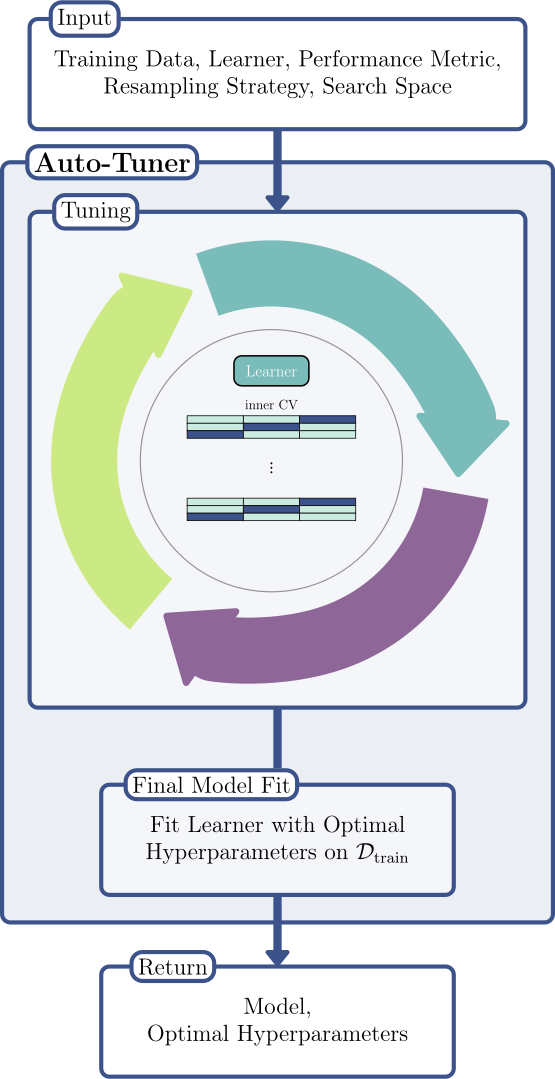
\includegraphics[width=0.6\textwidth]{chapters/chapter4/Figures/mlr3book_figures-12.png}

}

\caption{\label{fig-auto-tuner}Illustration of an Auto-Tuner.}

\end{figure}

And we can now call \texttt{\$train()}, which will first tune the
hyperparameters in the search space listed above before fitting the
optimal model.

\begin{Shaded}
\begin{Highlighting}[]
\NormalTok{split }\OtherTok{=} \FunctionTok{partition}\NormalTok{(tsk\_sonar)}
\NormalTok{at}\SpecialCharTok{$}\FunctionTok{train}\NormalTok{(tsk\_sonar, }\AttributeTok{row\_ids =}\NormalTok{ split}\SpecialCharTok{$}\NormalTok{train)}
\NormalTok{at}\SpecialCharTok{$}\FunctionTok{predict}\NormalTok{(tsk\_sonar, }\AttributeTok{row\_ids =}\NormalTok{ split}\SpecialCharTok{$}\NormalTok{test)}\SpecialCharTok{$}\FunctionTok{score}\NormalTok{()}
\end{Highlighting}
\end{Shaded}

\begin{verbatim}
classif.ce 
    0.2029 
\end{verbatim}

The \texttt{AutoTuner} contains a tuning instance that can be analyzed
like any other instance.

\begin{Shaded}
\begin{Highlighting}[]
\NormalTok{at}\SpecialCharTok{$}\NormalTok{tuning\_instance}\SpecialCharTok{$}\NormalTok{result}
\end{Highlighting}
\end{Shaded}

\begin{verbatim}
    cost  gamma learner_param_vals  x_domain classif.ce
1: 5.756 -5.756          <list[4]> <list[2]>     0.1727
\end{verbatim}

We could also pass the \texttt{AutoTuner} to
\href{https://mlr3.mlr-org.com/reference/resample.html}{\texttt{resample()}}
and
\href{https://mlr3.mlr-org.com/reference/benchmark.html}{\texttt{benchmark()}},
which would result in a nested resampling, discussed next.

\hypertarget{sec-nested-resampling}{%
\section{Nested Resampling}\label{sec-nested-resampling}}

HPO requires additional resampling to reduce bias when estimating the
performance of a model. If the same data is used for determining the
optimal configuration and the evaluation of the resulting model itself,
the actual performance estimate might be biased (Simon 2007). This is
analogous to optimism of the training
error\index{optimism of the training error} described in James et al.
(2014), which occurs when training error is taken as an estimate of
out-of-sample performance.

Nested resampling\index{nested resampling} separates model optimization
from the process of estimating the performance of the tuned model by
adding an additional resampling, i.e., while model performance is
estimated using a resampling method in the `usual way', tuning is then
performed by resampling the resampled data
(Figure~\ref{fig-nested-resampling}). For more details and a formal
introduction to nested resampling the reader is referred to Bischl et
al. (2023) and Simon (2007).

\begin{figure}

{\centering 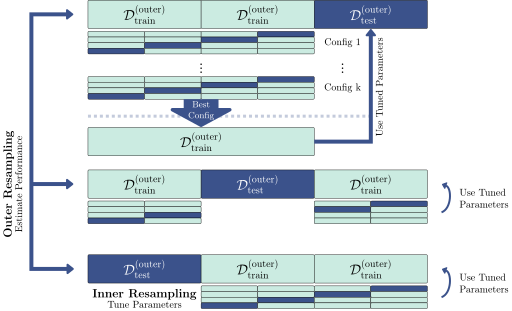
\includegraphics[width=0.8\textwidth,height=\textheight]{chapters/chapter4/Figures/mlr3book_figures-11.png}

}

\caption{\label{fig-nested-resampling}An illustration of nested
resampling. The large blocks represent three-fold CV for the outer
resampling for model evaluation and the small blocks represent four-fold
CV for the inner resampling for HPO. The light blue blocks are the
training sets and the dark blue blocks are the test sets.}

\end{figure}

Figure~\ref{fig-nested-resampling} represents the following example of
nested resampling:

\begin{enumerate}
\def\labelenumi{\arabic{enumi}.}
\tightlist
\item
  Outer resampling start -- Instantiate three-fold CV to create
  different testing and training datasets.
\item
  Inner resampling -- Within the outer training data instantiate
  four-fold CV to create different inner testing and training datasets.
\item
  HPO -- Tune the hyperparameters on the outer training set (large,
  light blue blocks) using the inner data splits.
\item
  Training -- Fit the learner on the outer training dataset using the
  optimal hyperparameter configuration obtained from the inner
  resampling (small blocks).
\item
  Evaluation -- Evaluate the performance of the learner on the outer
  testing data (large, dark blue block).
\item
  Outer resampling repeats -- Repeat (2)-(5) for each of the three outer
  folds.
\item
  Aggregation -- Take the sample mean of the three performance values
  for an unbiased performance estimate.
\end{enumerate}

The inner resampling produces generalization performance estimates for
each configuration and selects the optimal configuration to be evaluated
on the outer resampling. The outer resampling then produces
generalization estimates for these optimal configurations. The result
from the outer resampling can be used for comparison to other models
trained and tested on the same outer folds.

\begin{tcolorbox}[enhanced jigsaw, opacitybacktitle=0.6, rightrule=.15mm, opacityback=0, arc=.35mm, breakable, titlerule=0mm, colframe=quarto-callout-tip-color-frame, coltitle=black, bottomrule=.15mm, toprule=.15mm, colback=white, colbacktitle=quarto-callout-tip-color!10!white, bottomtitle=1mm, toptitle=1mm, title=\textcolor{quarto-callout-tip-color}{\faLightbulb}\hspace{0.5em}{Nested Resampling and Parallelization}, leftrule=.75mm, left=2mm]

Nested resampling is computationally expensive, three outer folds and
four inner folds with a grid search of resolution five used to tune two
parameters, results in \(3*4*5^2 = 300\) iterations of model
training/testing. If you have the resources we recommend utilizing
parallelization when tuning (Section~\ref{sec-parallelization}).

\end{tcolorbox}

A common mistake is to think of nested resampling as a method to select
optimal model configurations. Nested resampling is a method to compare
models and to estimate the generalization performance of a tuned model,
however, this is the performance based on multiple different
configurations (one from each outer fold) and not performance based on a
\emph{single} configuration (Section~\ref{sec-resample-overfitting}). If
you are interested in identifying optimal configurations, then use
\href{https://mlr3tuning.mlr-org.com/reference/tune.html}{\texttt{tune()}}\index{\texttt{tune()}}/\href{https://mlr3tuning.mlr-org.com/reference/ti.html}{\texttt{ti()}}
or
\href{https://mlr3tuning.mlr-org.com/reference/auto_tuner.html}{\texttt{auto\_tuner()}}\index{\texttt{auto\_tuner()}}
with \texttt{\$train()} on the complete dataset.

\hypertarget{nested-resampling-with-an-autotuner}{%
\subsection{\texorpdfstring{Nested Resampling with an
\texttt{AutoTuner}}{Nested Resampling with an AutoTuner}}\label{nested-resampling-with-an-autotuner}}

While the theory of nested resampling may seem complicated, it is all
automated in \texttt{mlr3tuning} by simply passing an \texttt{AutoTuner}
to
\href{https://mlr3.mlr-org.com/reference/resample.html}{\texttt{resample()}}
or
\href{https://mlr3.mlr-org.com/reference/benchmark.html}{\texttt{benchmark()}}.
Continuing with our previous example, we will use the auto-tuner to
resample a support vector classifier with three-fold CV in the outer
resampling and four-fold CV in the inner resampling.

\begin{Shaded}
\begin{Highlighting}[]
\NormalTok{at }\OtherTok{=} \FunctionTok{auto\_tuner}\NormalTok{(}
  \AttributeTok{tuner =}\NormalTok{ tnr\_grid\_search,}
  \AttributeTok{learner =}\NormalTok{ lrn\_svm,}
  \AttributeTok{resampling =} \FunctionTok{rsmp}\NormalTok{(}\StringTok{"cv"}\NormalTok{, }\AttributeTok{folds =} \DecValTok{4}\NormalTok{),}
  \AttributeTok{measure =}\NormalTok{ msr\_ce,}
\NormalTok{)}

\NormalTok{rr }\OtherTok{=} \FunctionTok{resample}\NormalTok{(tsk\_sonar, at, rsmp\_cv3, }\AttributeTok{store\_models =} \ConstantTok{TRUE}\NormalTok{)}

\NormalTok{rr}
\end{Highlighting}
\end{Shaded}

\begin{verbatim}
<ResampleResult> with 3 resampling iterations
 task_id        learner_id resampling_id iteration warnings errors
   sonar classif.svm.tuned            cv         1        0      0
   sonar classif.svm.tuned            cv         2        0      0
   sonar classif.svm.tuned            cv         3        0      0
\end{verbatim}

Note that we set \texttt{store\_models\ =\ TRUE} so that the
\texttt{AutoTuner} models (fitted on the outer training data) are
stored, which also enables investigation of the inner tuning instances.
While we used k-fold CV for both the inner and outer resampling
strategy, you could use different resampling strategies
(Section~\ref{sec-resampling}) and also different parallelization
methods (Section~\ref{sec-nested-resampling-parallelization}).

The estimated performance of a tuned model is reported as the aggregated
performance of all outer resampling iterations, which is a less biased
estimate of future model performance.

\begin{Shaded}
\begin{Highlighting}[]
\NormalTok{rr}\SpecialCharTok{$}\FunctionTok{aggregate}\NormalTok{()}
\end{Highlighting}
\end{Shaded}

\begin{verbatim}
classif.ce 
    0.1589 
\end{verbatim}

In addition to the methods described in Section~\ref{sec-resampling},
\href{https://mlr3tuning.mlr-org.com/reference/extract_inner_tuning_results.html}{\texttt{extract\_inner\_tuning\_results()}}
and
\href{https://mlr3tuning.mlr-org.com/reference/extract_inner_tuning_archives.html}{\texttt{extract\_inner\_tuning\_archives()}}
return the optimal configurations (across all outer folds) and full
tuning archives, respectively.

\begin{Shaded}
\begin{Highlighting}[]
\FunctionTok{extract\_inner\_tuning\_results}\NormalTok{(rr)[,}
\NormalTok{  .(iteration, cost, gamma, classif.ce)]}
\end{Highlighting}
\end{Shaded}

\begin{verbatim}
   iteration  cost  gamma classif.ce
1:         1 11.51 -5.756     0.2174
2:         2 11.51 -5.756     0.2086
3:         3 11.51 -5.756     0.1796
\end{verbatim}

\begin{Shaded}
\begin{Highlighting}[]
\FunctionTok{extract\_inner\_tuning\_archives}\NormalTok{(rr)[}\DecValTok{1}\SpecialCharTok{:}\DecValTok{3}\NormalTok{,}
\NormalTok{  .(iteration, cost, gamma, classif.ce)]}
\end{Highlighting}
\end{Shaded}

\begin{verbatim}
   iteration   cost   gamma classif.ce
1:         1 -11.51 -11.513     0.5286
2:         1 -11.51  11.513     0.5286
3:         1   0.00  -5.756     0.2981
\end{verbatim}

\hypertarget{sec-resample-overfitting}{%
\subsection{The Right (and Wrong) Way to Estimate
Performance}\label{sec-resample-overfitting}}

\begin{tcolorbox}[enhanced jigsaw, colframe=quarto-callout-note-color-frame, rightrule=.15mm, bottomrule=.15mm, toprule=.15mm, opacityback=0, colback=white, left=2mm, arc=.35mm, breakable, leftrule=.75mm]
\begin{minipage}[t]{5.5mm}
\textcolor{quarto-callout-note-color}{\faInfo}
\end{minipage}%
\begin{minipage}[t]{\textwidth - 5.5mm}

\textbf{This section covers advanced ML or technical
details.}\vspace{2mm}

\end{minipage}%
\end{tcolorbox}

In this short section we will empirically demonstrate that directly
reporting tuning performance without nested resampling results in
optimistically biased performance estimates. In this experiment we tune
several parameters from \texttt{lrn("classif.xgboost")}. To best
estimate the generalization performance we make use of the
\texttt{"moons"}
\href{https://mlr3.mlr-org.com/reference/TaskGenerator.html}{\texttt{TaskGenerator}}\index{\texttt{TaskGenerator}}{\marginnote{\begin{footnotesize}\texttt{TaskGenerator}\end{footnotesize}}}.
The \texttt{TaskGenerator} class is used when you want to simulate data
for use in experiments, these are very useful in cases such as this
experiment when you need access to an infinite number of data points to
estimate quantities such as the generalization error.

We begin by loading our learner, task generator, and generating 100
training data points and 1,000,000 testing data points.

\begin{Shaded}
\begin{Highlighting}[]
\NormalTok{lrn\_xgboost }\OtherTok{=} \FunctionTok{lrn}\NormalTok{(}\StringTok{"classif.xgboost"}\NormalTok{,}
  \AttributeTok{eta               =} \FunctionTok{to\_tune}\NormalTok{(}\FloatTok{1e{-}4}\NormalTok{, }\DecValTok{1}\NormalTok{, }\AttributeTok{logscale =} \ConstantTok{TRUE}\NormalTok{),}
  \AttributeTok{max\_depth         =} \FunctionTok{to\_tune}\NormalTok{(}\DecValTok{1}\NormalTok{, }\DecValTok{20}\NormalTok{),}
  \AttributeTok{colsample\_bytree  =} \FunctionTok{to\_tune}\NormalTok{(}\FloatTok{1e{-}1}\NormalTok{, }\DecValTok{1}\NormalTok{),}
  \AttributeTok{colsample\_bylevel =} \FunctionTok{to\_tune}\NormalTok{(}\FloatTok{1e{-}1}\NormalTok{, }\DecValTok{1}\NormalTok{),}
  \AttributeTok{lambda            =} \FunctionTok{to\_tune}\NormalTok{(}\FloatTok{1e{-}3}\NormalTok{, }\FloatTok{1e3}\NormalTok{, }\AttributeTok{logscale =} \ConstantTok{TRUE}\NormalTok{),}
  \AttributeTok{alpha             =} \FunctionTok{to\_tune}\NormalTok{(}\FloatTok{1e{-}3}\NormalTok{, }\FloatTok{1e3}\NormalTok{, }\AttributeTok{logscale =} \ConstantTok{TRUE}\NormalTok{),}
  \AttributeTok{subsample         =} \FunctionTok{to\_tune}\NormalTok{(}\FloatTok{1e{-}1}\NormalTok{, }\DecValTok{1}\NormalTok{)}
\NormalTok{)}
\NormalTok{tsk\_moons }\OtherTok{=} \FunctionTok{tgen}\NormalTok{(}\StringTok{"moons"}\NormalTok{)}
\NormalTok{tsk\_moons\_train }\OtherTok{=}\NormalTok{ tsk\_moons}\SpecialCharTok{$}\FunctionTok{generate}\NormalTok{(}\DecValTok{100}\NormalTok{)}
\NormalTok{tsk\_moons\_test }\OtherTok{=}\NormalTok{ tsk\_moons}\SpecialCharTok{$}\FunctionTok{generate}\NormalTok{(}\DecValTok{1000000}\NormalTok{)}
\end{Highlighting}
\end{Shaded}

Now we will tune the learner with respect to the classification error,
using holdout resampling and random search with 700 evaluations. We then
report the tuning performance without nested resampling.

\begin{Shaded}
\begin{Highlighting}[]
\NormalTok{tnr\_random }\OtherTok{=} \FunctionTok{tnr}\NormalTok{(}\StringTok{"random\_search"}\NormalTok{)}
\NormalTok{rsmp\_holdout }\OtherTok{=} \FunctionTok{rsmp}\NormalTok{(}\StringTok{"holdout"}\NormalTok{)}
\NormalTok{trm\_evals700 }\OtherTok{=} \FunctionTok{trm}\NormalTok{(}\StringTok{"evals"}\NormalTok{, }\AttributeTok{n\_evals =} \DecValTok{700}\NormalTok{)}

\NormalTok{instance }\OtherTok{=} \FunctionTok{tune}\NormalTok{(}
  \AttributeTok{tuner =}\NormalTok{ tnr\_random,}
  \AttributeTok{task =}\NormalTok{ tsk\_moons\_train,}
  \AttributeTok{learner =}\NormalTok{ lrn\_xgboost,}
  \AttributeTok{resampling =}\NormalTok{ rsmp\_holdout,}
  \AttributeTok{measures =}\NormalTok{ msr\_ce,}
  \AttributeTok{terminator =}\NormalTok{ trm\_evals700}
\NormalTok{)}

\NormalTok{insample }\OtherTok{=}\NormalTok{ instance}\SpecialCharTok{$}\NormalTok{result\_y}
\end{Highlighting}
\end{Shaded}

Next, we estimate generalization error by nested resampling (below we
use an outer five-fold CV), using an \texttt{AutoTuner}:

\begin{Shaded}
\begin{Highlighting}[]
\CommentTok{\# same setup as above}
\NormalTok{at }\OtherTok{=} \FunctionTok{auto\_tuner}\NormalTok{(}
  \AttributeTok{tuner =}\NormalTok{ tnr\_random,}
  \AttributeTok{learner =}\NormalTok{ lrn\_xgboost,}
  \AttributeTok{resampling =}\NormalTok{ rsmp\_holdout,}
  \AttributeTok{measure =}\NormalTok{ msr\_ce,}
  \AttributeTok{terminator =}\NormalTok{ trm\_evals700}
\NormalTok{)}

\NormalTok{rsmp\_cv5 }\OtherTok{=} \FunctionTok{rsmp}\NormalTok{(}\StringTok{"cv"}\NormalTok{, }\AttributeTok{folds =} \DecValTok{5}\NormalTok{)}

\NormalTok{outsample }\OtherTok{=} \FunctionTok{resample}\NormalTok{(tsk\_moons\_train, at, rsmp\_cv5)}\SpecialCharTok{$}\FunctionTok{aggregate}\NormalTok{()}
\end{Highlighting}
\end{Shaded}

And finally, we estimate the generalization
error\index{generalization error} by training the tuned learner (i.e.,
using the values from the \texttt{instance} above) on the full training
data again and predicting on the test data.

\begin{Shaded}
\begin{Highlighting}[]
\NormalTok{lrn\_xgboost\_tuned }\OtherTok{=} \FunctionTok{lrn}\NormalTok{(}\StringTok{"classif.xgboost"}\NormalTok{)}
\NormalTok{lrn\_xgboost\_tuned}\SpecialCharTok{$}\NormalTok{param\_set}\SpecialCharTok{$}\FunctionTok{set\_values}\NormalTok{(}
  \AttributeTok{.values =}\NormalTok{ instance}\SpecialCharTok{$}\NormalTok{result\_learner\_param\_vals)}
\NormalTok{generalization }\OtherTok{=}\NormalTok{ lrn\_xgboost\_tuned}\SpecialCharTok{$}\FunctionTok{train}\NormalTok{(tsk\_moons\_train)}\SpecialCharTok{$}
  \FunctionTok{predict}\NormalTok{(tsk\_moons\_test)}\SpecialCharTok{$}\FunctionTok{score}\NormalTok{()}
\end{Highlighting}
\end{Shaded}

Now we can compare these three values:

\begin{Shaded}
\begin{Highlighting}[]
\FunctionTok{round}\NormalTok{(}\FunctionTok{c}\NormalTok{(}\AttributeTok{true\_generalization =} \FunctionTok{as.numeric}\NormalTok{(generalization),}
  \AttributeTok{without\_nested\_resampling =} \FunctionTok{as.numeric}\NormalTok{(insample),}
  \AttributeTok{with\_nested\_resampling =} \FunctionTok{as.numeric}\NormalTok{(outsample)), }\DecValTok{2}\NormalTok{)}
\end{Highlighting}
\end{Shaded}

\begin{verbatim}
      true_generalization without_nested_resampling 
                     0.19                      0.06 
   with_nested_resampling 
                     0.22 
\end{verbatim}

We find that the performance estimate from unnested tuning
optimistically overestimates the true performance (which could indicate
`meta-overfitting' to the specific inner holdout-splits), while the
outer estimate from nested resampling works much better.

\hypertarget{sec-defining-search-spaces}{%
\section{More Advanced Search Spaces}\label{sec-defining-search-spaces}}

Up until now, we have only considered tuning simple search spaces
limited to a few numeric hyperparameters. In this section, we will first
look at how to tune different scalar parameter classes with
\href{https://paradox.mlr-org.com/reference/to_tune.html}{\texttt{to\_tune()}},
and then how to define your own search space with
\href{https://paradox.mlr-org.com/reference/ParamSet.html}{\texttt{ParamSet}}
to create more advanced search spaces that may include tuning over
vectors, transformations, and handling parameter dependencies. Finally,
we will consider how to access a database of standardized search spaces
from the literature.

\hypertarget{scalar-parameter-tuning}{%
\subsection{Scalar Parameter Tuning}\label{scalar-parameter-tuning}}

The
\href{https://paradox.mlr-org.com/reference/to_tune.html}{\texttt{to\_tune()}}
function can be used to tune parameters of any class, whether they are
scalar or vectors. To best understand this function, we will consider
what is happening behind the scenes. When \texttt{to\_tune()} is used in
a learner, implicitly a
\href{https://paradox.mlr-org.com/reference/ParamSet.html}{\texttt{ParamSet}}
is created just for the tuning search space:

\begin{Shaded}
\begin{Highlighting}[]
\NormalTok{learner }\OtherTok{=} \FunctionTok{lrn}\NormalTok{(}\StringTok{"classif.svm"}\NormalTok{,}
  \AttributeTok{cost  =} \FunctionTok{to\_tune}\NormalTok{(}\FloatTok{1e{-}1}\NormalTok{, }\FloatTok{1e5}\NormalTok{),}
  \AttributeTok{gamma =} \FunctionTok{to\_tune}\NormalTok{(}\FloatTok{1e{-}1}\NormalTok{, }\DecValTok{1}\NormalTok{),}
  \AttributeTok{kernel =} \StringTok{"radial"}\NormalTok{,}
  \AttributeTok{type =} \StringTok{"C{-}classification"}
\NormalTok{)}

\NormalTok{learner}\SpecialCharTok{$}\NormalTok{param\_set}\SpecialCharTok{$}\FunctionTok{search\_space}\NormalTok{()}
\end{Highlighting}
\end{Shaded}

\begin{verbatim}
<ParamSet>
      id    class lower upper nlevels        default value
1:  cost ParamDbl   0.1 1e+05     Inf <NoDefault[3]>      
2: gamma ParamDbl   0.1 1e+00     Inf <NoDefault[3]>      
\end{verbatim}

Recall from Section~\ref{sec-param-set}, that the \texttt{class} field
corresponds to the hyperparameter class as defined in
\href{https://paradox.mlr-org.com}{\texttt{paradox}}. In this example,
we can see that \texttt{gamma} hyperparameter has class
\href{https://paradox.mlr-org.com/reference/ParamDbl.html}{\texttt{ParamDbl}},
with \texttt{lower\ =\ 0.1} and \texttt{upper\ =\ 1}, which was
automatically created by \texttt{to\_tune()} as we passed two numeric
values to this function. If we wanted to tune over a non-numeric
hyperparameter, we can still use \texttt{to\_tune()}, which will infer
the correct class to construct in the resulting parameter set. For
example, say we wanted to tune the numeric \texttt{cost}, factor
\texttt{kernel}, and logical \texttt{scale} hyperparameter in our SVM:

\begin{Shaded}
\begin{Highlighting}[]
\NormalTok{learner }\OtherTok{=} \FunctionTok{lrn}\NormalTok{(}\StringTok{"classif.svm"}\NormalTok{,}
  \AttributeTok{cost  =} \FunctionTok{to\_tune}\NormalTok{(}\FloatTok{1e{-}1}\NormalTok{, }\FloatTok{1e5}\NormalTok{),}
  \AttributeTok{kernel =} \FunctionTok{to\_tune}\NormalTok{(}\FunctionTok{c}\NormalTok{(}\StringTok{"radial"}\NormalTok{, }\StringTok{"linear"}\NormalTok{)),}
  \AttributeTok{shrinking =} \FunctionTok{to\_tune}\NormalTok{(),}
  \AttributeTok{type =} \StringTok{"C{-}classification"}
\NormalTok{)}

\NormalTok{learner}\SpecialCharTok{$}\NormalTok{param\_set}\SpecialCharTok{$}\FunctionTok{search\_space}\NormalTok{()}
\end{Highlighting}
\end{Shaded}

\begin{verbatim}
<ParamSet>
          id    class lower upper nlevels        default value
1:      cost ParamDbl   0.1 1e+05     Inf <NoDefault[3]>      
2:    kernel ParamFct    NA    NA       2 <NoDefault[3]>      
3: shrinking ParamLgl    NA    NA       2           TRUE      
\end{verbatim}

Here the \texttt{kernel} hyperparameter is a factor, so we simply pass
in a vector corresponding to the levels we want to tune over. The
\texttt{shrinking} hyperparameter is a logical, there are only two
possible values this could take so we do not need to pass anything to
\texttt{to\_tune()}, it will automatically recognize this is a logical
from \texttt{learner\$param\_set} and passes this detail to
\texttt{learner\$param\_set\$search\_space()}. Similarly, for factor
parameters, we could also use \texttt{to\_tune()} without any arguments
if we want to tune over all possible values. Finally, we can use
\texttt{to\_tune()} to treat numeric parameters as factors if we want to
discretize them over a small subset of possible values, for example, if
we wanted to find the optimal number of trees in a random forest we
might only consider three scenarios: 100, 200, or 400 trees:

\begin{Shaded}
\begin{Highlighting}[]
\FunctionTok{lrn}\NormalTok{(}\StringTok{"classif.ranger"}\NormalTok{, }\AttributeTok{num.trees =} \FunctionTok{to\_tune}\NormalTok{(}\FunctionTok{c}\NormalTok{(}\DecValTok{100}\NormalTok{, }\DecValTok{200}\NormalTok{, }\DecValTok{400}\NormalTok{)))}
\end{Highlighting}
\end{Shaded}

Before we look at tuning over vectors, we must first learn how to create
parameter sets from scratch.

\begin{tcolorbox}[enhanced jigsaw, opacitybacktitle=0.6, rightrule=.15mm, opacityback=0, arc=.35mm, breakable, titlerule=0mm, colframe=quarto-callout-warning-color-frame, coltitle=black, bottomrule=.15mm, toprule=.15mm, colback=white, colbacktitle=quarto-callout-warning-color!10!white, bottomtitle=1mm, toptitle=1mm, title=\textcolor{quarto-callout-warning-color}{\faExclamationTriangle}\hspace{0.5em}{Ordered Hyperparameters}, leftrule=.75mm, left=2mm]

Treating an integer as a factor for tuning results in ``unordered''
hyperparameters. Therefore algorithms that make use of ordering
information will perform worse when ordering is ignored. For these
algorithms, it would make more sense to define a
\href{https://paradox.mlr-org.com/reference/ParamDbl.html}{\texttt{ParamDbl}}
or
\href{https://paradox.mlr-org.com/reference/ParamInt.html}{\texttt{ParamInt}}
(Section~\ref{sec-tune-ps}) with a custom transformation
(Section~\ref{sec-tune-trafo}).

\end{tcolorbox}

\hypertarget{sec-tune-ps}{%
\subsection{\texorpdfstring{Defining Search Spaces with
\texttt{ps}}{Defining Search Spaces with ps}}\label{sec-tune-ps}}

As we have seen,
\href{https://paradox.mlr-org.com/reference/to_tune.html}{\texttt{to\_tune()}}
is a helper function that creates a parameter set that will go on to be
used by
\href{https://mlr3tuning.mlr-org.com/reference/tune.html}{\texttt{tune()}},
\href{https://mlr3tuning.mlr-org.com/reference/ti.html}{\texttt{ti()}},
or
\href{https://mlr3tuning.mlr-org.com/reference/auto_tuner.html}{\texttt{auto\_tuner()}}
during the tuning process. However, there will be use cases where you
will need to create a parameter set manually using
\href{https://paradox.mlr-org.com/reference/ps.html}{\texttt{ps()}}.
This function takes named arguments of class
\href{https://paradox.mlr-org.com/reference/Param.html}{\texttt{Param}},
which can be created using the sugar functions in
Table~\ref{tbl-paradox-define}.

\hypertarget{tbl-paradox-define}{}
\begin{longtable}[]{@{}
  >{\raggedright\arraybackslash}p{(\columnwidth - 4\tabcolsep) * \real{0.2338}}
  >{\raggedright\arraybackslash}p{(\columnwidth - 4\tabcolsep) * \real{0.4935}}
  >{\raggedright\arraybackslash}p{(\columnwidth - 4\tabcolsep) * \real{0.2727}}@{}}
\caption{\label{tbl-paradox-define}\href{https://paradox.mlr-org.com/reference/Domain.html}{\texttt{Domain}}
Constructors and their resulting
\href{https://paradox.mlr-org.com/reference/Param.html}{\texttt{Param}}.}\tabularnewline
\toprule\noalign{}
\begin{minipage}[b]{\linewidth}\raggedright
Constructor
\end{minipage} & \begin{minipage}[b]{\linewidth}\raggedright
Description
\end{minipage} & \begin{minipage}[b]{\linewidth}\raggedright
Underlying Class
\end{minipage} \\
\midrule\noalign{}
\endfirsthead
\toprule\noalign{}
\begin{minipage}[b]{\linewidth}\raggedright
Constructor
\end{minipage} & \begin{minipage}[b]{\linewidth}\raggedright
Description
\end{minipage} & \begin{minipage}[b]{\linewidth}\raggedright
Underlying Class
\end{minipage} \\
\midrule\noalign{}
\endhead
\bottomrule\noalign{}
\endlastfoot
\href{https://paradox.mlr-org.com/reference/Domain.html}{\texttt{p\_dbl}}
& Real valued parameter (``double'') &
\href{https://paradox.mlr-org.com/reference/ParamDbl.html}{\texttt{ParamDbl}} \\
\href{https://paradox.mlr-org.com/reference/Domain.html}{\texttt{p\_int}}
& Integer parameter &
\href{https://paradox.mlr-org.com/reference/ParamInt.html}{\texttt{ParamInt}} \\
\href{https://paradox.mlr-org.com/reference/Domain.html}{\texttt{p\_fct}}
& Discrete valued parameter (``factor'') &
\href{https://paradox.mlr-org.com/reference/ParamFct.html}{\texttt{ParamFct}} \\
\href{https://paradox.mlr-org.com/reference/Domain.html}{\texttt{p\_lgl}}
& Logical / Boolean parameter &
\href{https://paradox.mlr-org.com/reference/ParamLgl.html}{\texttt{ParamLgl}} \\
\href{https://paradox.mlr-org.com/reference/Domain.html}{\texttt{p\_uty}}
& Untyped parameter &
\href{https://paradox.mlr-org.com/reference/ParamUty.html}{\texttt{ParamUty}} \\
\end{longtable}

As a simple example, let us look at how to create a search space to tune
\texttt{cost} and \texttt{gamma} again:

\begin{Shaded}
\begin{Highlighting}[]
\NormalTok{search\_space }\OtherTok{=} \FunctionTok{ps}\NormalTok{(}
  \AttributeTok{cost  =} \FunctionTok{p\_dbl}\NormalTok{(}\AttributeTok{lower =} \FloatTok{1e{-}1}\NormalTok{, }\AttributeTok{upper =} \FloatTok{1e5}\NormalTok{),}
  \AttributeTok{kernel =} \FunctionTok{p\_fct}\NormalTok{(}\FunctionTok{c}\NormalTok{(}\StringTok{"radial"}\NormalTok{, }\StringTok{"linear"}\NormalTok{)),}
  \AttributeTok{shrinking =} \FunctionTok{p\_lgl}\NormalTok{()}
\NormalTok{)}
\end{Highlighting}
\end{Shaded}

This search space would then be passed to the \texttt{search\_space}
argument in \texttt{auto\_tuner()}:

\begin{Shaded}
\begin{Highlighting}[]
\FunctionTok{ti}\NormalTok{(tsk\_sonar, }\FunctionTok{lrn}\NormalTok{(}\StringTok{"classif.svm"}\NormalTok{, }\AttributeTok{type =} \StringTok{"C{-}classification"}\NormalTok{), rsmp\_cv3,}
\NormalTok{  msr\_ce, }\FunctionTok{trm}\NormalTok{(}\StringTok{"none"}\NormalTok{), }\AttributeTok{search\_space =}\NormalTok{ search\_space)}
\end{Highlighting}
\end{Shaded}

\begin{verbatim}
<TuningInstanceSingleCrit>
* State:  Not optimized
* Objective: <ObjectiveTuning:classif.svm_on_sonar>
* Search Space:
          id    class lower upper nlevels
1:      cost ParamDbl   0.1 1e+05     Inf
2:    kernel ParamFct    NA    NA       2
3: shrinking ParamLgl    NA    NA       2
* Terminator: <TerminatorNone>
\end{verbatim}

\begin{tcolorbox}[enhanced jigsaw, opacitybacktitle=0.6, rightrule=.15mm, opacityback=0, arc=.35mm, breakable, titlerule=0mm, colframe=quarto-callout-warning-color-frame, coltitle=black, bottomrule=.15mm, toprule=.15mm, colback=white, colbacktitle=quarto-callout-warning-color!10!white, bottomtitle=1mm, toptitle=1mm, title=\textcolor{quarto-callout-warning-color}{\faExclamationTriangle}\hspace{0.5em}{Bounded Search Spaces}, leftrule=.75mm, left=2mm]

When manually creating search spaces, make sure all numeric
hyperparameters in your search space are bounded, e.g., if you are
trying to tune a hyperparameter that could take any value in
\((-\infty, \infty)\) then the tuning process will throw an error for
nearly all tuners if you do not pass lower and upper limits to
\texttt{p\_dbl()} or \texttt{p\_int()}. You can use
\texttt{\$is\_bounded} on the constructed
\href{https://paradox.mlr-org.com/reference/ParamSet.html}{\texttt{ParamSet}}
if you are unsure:

\begin{Shaded}
\begin{Highlighting}[]
\FunctionTok{ps}\NormalTok{(}\AttributeTok{cost =} \FunctionTok{p\_dbl}\NormalTok{(}\AttributeTok{lower =} \FloatTok{0.1}\NormalTok{, }\AttributeTok{upper =} \DecValTok{1}\NormalTok{))}\SpecialCharTok{$}\NormalTok{is\_bounded}
\end{Highlighting}
\end{Shaded}

\begin{verbatim}
[1] TRUE
\end{verbatim}

\begin{Shaded}
\begin{Highlighting}[]
\FunctionTok{ps}\NormalTok{(}\AttributeTok{cost =} \FunctionTok{p\_dbl}\NormalTok{(}\AttributeTok{lower =} \FloatTok{0.1}\NormalTok{, }\AttributeTok{upper =} \ConstantTok{Inf}\NormalTok{))}\SpecialCharTok{$}\NormalTok{is\_bounded}
\end{Highlighting}
\end{Shaded}

\begin{verbatim}
[1] FALSE
\end{verbatim}

\end{tcolorbox}

\hypertarget{sec-tune-trafo}{%
\subsection{Transformations and Tuning Over
Vectors}\label{sec-tune-trafo}}

\begin{tcolorbox}[enhanced jigsaw, colframe=quarto-callout-note-color-frame, rightrule=.15mm, bottomrule=.15mm, toprule=.15mm, opacityback=0, colback=white, left=2mm, arc=.35mm, breakable, leftrule=.75mm]
\begin{minipage}[t]{5.5mm}
\textcolor{quarto-callout-note-color}{\faInfo}
\end{minipage}%
\begin{minipage}[t]{\textwidth - 5.5mm}

\textbf{This section covers advanced ML or technical
details.}\vspace{2mm}

\end{minipage}%
\end{tcolorbox}

In Section~\ref{sec-logarithmic-transformations} we saw how to quickly
apply log transformations with
\href{https://paradox.mlr-org.com/reference/to_tune.html}{\texttt{to\_tune()}}.
As you now know, \texttt{to\_tune()} is just a wrapper that creates
\href{https://paradox.mlr-org.com/reference/ParamSet.html}{\texttt{ParamSet}}
objects, so let us look at what is taking place when we set
\texttt{logscale\ =\ TRUE}:

\begin{Shaded}
\begin{Highlighting}[]
\FunctionTok{lrn}\NormalTok{(}\StringTok{"classif.svm"}\NormalTok{, }\AttributeTok{cost =} \FunctionTok{to\_tune}\NormalTok{(}\FloatTok{1e{-}5}\NormalTok{, }\FloatTok{1e5}\NormalTok{, }\AttributeTok{logscale =} \ConstantTok{TRUE}\NormalTok{))}\SpecialCharTok{$}
\NormalTok{  param\_set}\SpecialCharTok{$}\FunctionTok{search\_space}\NormalTok{()}
\end{Highlighting}
\end{Shaded}

\begin{verbatim}
<ParamSet>
     id    class  lower upper nlevels        default value
1: cost ParamDbl -11.51 11.51     Inf <NoDefault[3]>      
Trafo is set.
\end{verbatim}

Notice that now the \texttt{lower} and \texttt{upper} fields correspond
to the transformed bounds, i.e.~\([\log(1e-5), \log(1e5)]\). To manually
create the same transformation, we can pass the transformation to the
\texttt{trafo} argument in \texttt{p\_dbl()} and set the bounds:

\begin{Shaded}
\begin{Highlighting}[]
\NormalTok{search\_space }\OtherTok{=} \FunctionTok{ps}\NormalTok{(}\AttributeTok{cost =} \FunctionTok{p\_dbl}\NormalTok{(}\FunctionTok{log}\NormalTok{(}\FloatTok{1e{-}5}\NormalTok{), }\FunctionTok{log}\NormalTok{(}\FloatTok{1e5}\NormalTok{),}
  \AttributeTok{trafo =} \ControlFlowTok{function}\NormalTok{(x) }\FunctionTok{exp}\NormalTok{(x))) }\CommentTok{\# alternatively: \textquotesingle{}trafo = exp\textquotesingle{}}
\NormalTok{search\_space}
\end{Highlighting}
\end{Shaded}

\begin{verbatim}
<ParamSet>
     id    class  lower upper nlevels        default value
1: cost ParamDbl -11.51 11.51     Inf <NoDefault[3]>      
Trafo is set.
\end{verbatim}

We can confirm it is correctly set by making use of the
\texttt{\$trafo()} method, which takes a named list and applies the
specified transformations

\begin{Shaded}
\begin{Highlighting}[]
\NormalTok{search\_space}\SpecialCharTok{$}\FunctionTok{trafo}\NormalTok{(}\FunctionTok{list}\NormalTok{(}\AttributeTok{cost =} \DecValTok{1}\NormalTok{))}
\end{Highlighting}
\end{Shaded}

\begin{verbatim}
$cost
[1] 2.718
\end{verbatim}

Where transformations become the most powerful is in the ability to pass
arbitrary functions that can act on single parameters or even the entire
parameter set. As an example, consider a simple transformation to add
`2' to our range:

\begin{Shaded}
\begin{Highlighting}[]
\NormalTok{search\_space }\OtherTok{=} \FunctionTok{ps}\NormalTok{(}\AttributeTok{cost =} \FunctionTok{p\_dbl}\NormalTok{(}\DecValTok{0}\NormalTok{, }\DecValTok{3}\NormalTok{, }\AttributeTok{trafo =} \ControlFlowTok{function}\NormalTok{(x) x }\SpecialCharTok{+} \DecValTok{2}\NormalTok{))}
\NormalTok{search\_space}\SpecialCharTok{$}\FunctionTok{trafo}\NormalTok{(}\FunctionTok{list}\NormalTok{(}\AttributeTok{cost =} \DecValTok{1}\NormalTok{))}
\end{Highlighting}
\end{Shaded}

\begin{verbatim}
$cost
[1] 3
\end{verbatim}

Simple transformations such as this can even be added directly to a
learner by passing a \texttt{Param} object to \texttt{to\_tune()}:

\begin{Shaded}
\begin{Highlighting}[]
\FunctionTok{lrn}\NormalTok{(}\StringTok{"classif.svm"}\NormalTok{,}
  \AttributeTok{cost =} \FunctionTok{to\_tune}\NormalTok{(}\FunctionTok{p\_dbl}\NormalTok{(}\DecValTok{0}\NormalTok{, }\DecValTok{3}\NormalTok{, }\AttributeTok{trafo =} \ControlFlowTok{function}\NormalTok{(x) x }\SpecialCharTok{+} \DecValTok{2}\NormalTok{)))}
\end{Highlighting}
\end{Shaded}

More complex transformations that require multiple arguments should be
passed to the \texttt{.extra\_trafo} parameter in \texttt{ps()}.
\texttt{.extra\_trafo} takes a function with parameters \texttt{x} and
\texttt{param\_set} where, during tuning, \texttt{x} will be a list
containing the configuration being tested, and \texttt{param\_set} is
the whole parameter set. Below we first exponentiate the value of
\texttt{cost} and then add `2' if the \texttt{kernel} is
\texttt{"polynomial"}.

\begin{Shaded}
\begin{Highlighting}[]
\NormalTok{search\_space }\OtherTok{=} \FunctionTok{ps}\NormalTok{(}
  \AttributeTok{cost =} \FunctionTok{p\_dbl}\NormalTok{(}\SpecialCharTok{{-}}\DecValTok{1}\NormalTok{, }\DecValTok{1}\NormalTok{, }\AttributeTok{trafo =} \ControlFlowTok{function}\NormalTok{(x) }\FunctionTok{exp}\NormalTok{(x)),}
  \AttributeTok{kernel =} \FunctionTok{p\_fct}\NormalTok{(}\FunctionTok{c}\NormalTok{(}\StringTok{"polynomial"}\NormalTok{, }\StringTok{"radial"}\NormalTok{)),}
  \AttributeTok{.extra\_trafo =} \ControlFlowTok{function}\NormalTok{(x, param\_set) \{}
    \ControlFlowTok{if}\NormalTok{ (x}\SpecialCharTok{$}\NormalTok{kernel }\SpecialCharTok{==} \StringTok{"polynomial"}\NormalTok{) \{}
\NormalTok{      x}\SpecialCharTok{$}\NormalTok{cost }\OtherTok{=}\NormalTok{ x}\SpecialCharTok{$}\NormalTok{cost }\SpecialCharTok{+} \DecValTok{2}
\NormalTok{    \}}
\NormalTok{    x}
\NormalTok{  \}}
\NormalTok{)}
\NormalTok{search\_space}\SpecialCharTok{$}\FunctionTok{trafo}\NormalTok{(}\FunctionTok{list}\NormalTok{(}\AttributeTok{cost =} \DecValTok{1}\NormalTok{, }\AttributeTok{kernel =} \StringTok{"radial"}\NormalTok{))}
\end{Highlighting}
\end{Shaded}

\begin{verbatim}
$cost
[1] 2.718

$kernel
[1] "radial"
\end{verbatim}

\begin{Shaded}
\begin{Highlighting}[]
\NormalTok{search\_space}\SpecialCharTok{$}\FunctionTok{trafo}\NormalTok{(}\FunctionTok{list}\NormalTok{(}\AttributeTok{cost =} \DecValTok{1}\NormalTok{, }\AttributeTok{kernel =} \StringTok{"polynomial"}\NormalTok{))}
\end{Highlighting}
\end{Shaded}

\begin{verbatim}
$cost
[1] 4.718

$kernel
[1] "polynomial"
\end{verbatim}

\hypertarget{vector-transformations}{%
\subsubsection*{Vector transformations}\label{vector-transformations}}

Any function can be passed to \texttt{trafo} and \texttt{.extra\_trafo},
which enables tuning of `untyped' parameters of class
\href{https://paradox.mlr-org.com/reference/ParamUty.html}{\texttt{ParamUty}}
that could be vectors, functions, or any non-atomic class. By example,
consider the \texttt{class.weights} parameter of the SVM, which takes a
named vector of class weights with one entry for each target class. To
tune this parameter we could tune a scalar and then transform this to a
vector. The code below would result in a value, \texttt{x}, between
\texttt{0.1} and \texttt{0.9} being sampled, the result is then
transformed to (\texttt{x}, \texttt{1\ -\ x}) and is then passed to the
\texttt{Learner}.

\begin{Shaded}
\begin{Highlighting}[]
\NormalTok{search\_space }\OtherTok{=} \FunctionTok{ps}\NormalTok{(}
  \AttributeTok{class.weights =} \FunctionTok{p\_dbl}\NormalTok{(}\AttributeTok{lower =} \FloatTok{0.1}\NormalTok{, }\AttributeTok{upper =} \FloatTok{0.9}\NormalTok{,}
    \AttributeTok{trafo =} \ControlFlowTok{function}\NormalTok{(x) }\FunctionTok{c}\NormalTok{(}\AttributeTok{M =}\NormalTok{ x, }\AttributeTok{R =} \DecValTok{1} \SpecialCharTok{{-}}\NormalTok{ x))}
\NormalTok{)}
\end{Highlighting}
\end{Shaded}

In other cases, we may need to tune two or more `pseudoparameters' that
do not exist in our learner's parameter set but are required to tune a
vector parameter. For example, say we want to tune the architecture of a
neural network\index{neural network}, in which we need to decide the
number of layers and the number of nodes in each layer, this is the case
in the \texttt{num\_nodes} hyperparameter in
\texttt{lrn("surv.coxtime")} (we use this learner as it provides a
useful template for this sort of transformation, interested readers can
read about survival analysis in Section~\ref{sec-survival}). In this
case, the learner expects a vector where each element of the vector
corresponds to the number of nodes in a layer and the length of the
vector is the number of layers. We could then tune this as follows:

\begin{Shaded}
\begin{Highlighting}[]
\NormalTok{search\_space }\OtherTok{=} \FunctionTok{ps}\NormalTok{(}
  \AttributeTok{num\_layers =} \FunctionTok{p\_int}\NormalTok{(}\AttributeTok{lower =} \DecValTok{1}\NormalTok{, }\AttributeTok{upper =} \DecValTok{20}\NormalTok{),}
  \AttributeTok{num\_nodes\_per\_layer =} \FunctionTok{p\_int}\NormalTok{(}\DecValTok{4}\NormalTok{, }\DecValTok{64}\NormalTok{),}
  \AttributeTok{.extra\_trafo =} \ControlFlowTok{function}\NormalTok{(x, param\_set) \{}
\NormalTok{    x}\SpecialCharTok{$}\NormalTok{num\_nodes }\OtherTok{=} \FunctionTok{rep}\NormalTok{(x}\SpecialCharTok{$}\NormalTok{num\_nodes\_per\_layer, x}\SpecialCharTok{$}\NormalTok{num\_layers)}
\NormalTok{    x}\SpecialCharTok{$}\NormalTok{num\_layers }\OtherTok{=} \ConstantTok{NULL}
\NormalTok{    x}\SpecialCharTok{$}\NormalTok{num\_nodes\_per\_layer }\OtherTok{=} \ConstantTok{NULL}
\NormalTok{    x}
\NormalTok{  \}}
\NormalTok{)}
\end{Highlighting}
\end{Shaded}

Here we are tuning the pseudo-parameter \texttt{num\_layers} between
\texttt{1} and \texttt{20}, then tuning the pseudo-parameter
\texttt{num\_nodes\_per\_layer} between \texttt{4} and \texttt{64}, then
combining these into a vector called \texttt{num\_nodes} (the real
hyperparameter) and removing the pseudo-parameters.

\begin{Shaded}
\begin{Highlighting}[]
\NormalTok{search\_space}\SpecialCharTok{$}\FunctionTok{trafo}\NormalTok{(}\FunctionTok{list}\NormalTok{(}\AttributeTok{num\_layers =} \DecValTok{4}\NormalTok{, }\AttributeTok{num\_nodes\_per\_layer =} \DecValTok{12}\NormalTok{))}
\end{Highlighting}
\end{Shaded}

\begin{verbatim}
$num_nodes
[1] 12 12 12 12
\end{verbatim}

Even though this transformation looks complex, it only affects one of
the hyperparameters (and does not need access to others), so we could
include it in the learner using \texttt{to\_tune()} by passing the whole
\texttt{ParamSet} object:

\begin{Shaded}
\begin{Highlighting}[]
\NormalTok{learner }\OtherTok{=} \FunctionTok{lrn}\NormalTok{(}\StringTok{"surv.coxtime"}\NormalTok{)}
\NormalTok{learner}\SpecialCharTok{$}\NormalTok{param\_set}\SpecialCharTok{$}\FunctionTok{set\_values}\NormalTok{(}\AttributeTok{num\_nodes =} \FunctionTok{to\_tune}\NormalTok{(search\_space))}
\NormalTok{learner}\SpecialCharTok{$}\NormalTok{param\_set}\SpecialCharTok{$}\FunctionTok{search\_space}\NormalTok{()}
\end{Highlighting}
\end{Shaded}

\begin{verbatim}
<ParamSet>
                    id    class lower upper nlevels        default
1:          num_layers ParamInt     1    20      20 <NoDefault[3]>
2: num_nodes_per_layer ParamInt     4    64      61 <NoDefault[3]>
1 variable not shown: [value]
Trafo is set.
\end{verbatim}

\hypertarget{sec-optimization-depends}{%
\subsection{Hyperparameter
Dependencies}\label{sec-optimization-depends}}

\begin{tcolorbox}[enhanced jigsaw, colframe=quarto-callout-note-color-frame, rightrule=.15mm, bottomrule=.15mm, toprule=.15mm, opacityback=0, colback=white, left=2mm, arc=.35mm, breakable, leftrule=.75mm]
\begin{minipage}[t]{5.5mm}
\textcolor{quarto-callout-note-color}{\faInfo}
\end{minipage}%
\begin{minipage}[t]{\textwidth - 5.5mm}

\textbf{This section covers advanced ML or technical
details.}\vspace{2mm}

\end{minipage}%
\end{tcolorbox}

Hyperparameter dependencies occur when a hyperparameter should only be
set if another hyperparameter has a particular value. For example, the
\texttt{degree} parameter in SVM is only valid when \texttt{kernel} is
\texttt{"polynomial"}. In the
\href{https://paradox.mlr-org.com/reference/ps.html}{\texttt{ps()}}
function, we specify this using the \texttt{depends} argument, which
takes a named argument of the form
\texttt{\textless{}param\textgreater{}\ ==\ value} or
\texttt{\textless{}param\textgreater{}\ \%in\%\ \textless{}vector\textgreater{}}:

\begin{Shaded}
\begin{Highlighting}[]
\FunctionTok{ps}\NormalTok{(}
  \AttributeTok{kernel =} \FunctionTok{p\_fct}\NormalTok{(}\FunctionTok{c}\NormalTok{(}\StringTok{"polynomial"}\NormalTok{, }\StringTok{"radial"}\NormalTok{)),}
  \AttributeTok{degree =} \FunctionTok{p\_int}\NormalTok{(}\DecValTok{1}\NormalTok{, }\DecValTok{3}\NormalTok{, }\AttributeTok{depends =}\NormalTok{ (kernel }\SpecialCharTok{==} \StringTok{"polynomial"}\NormalTok{)),}
  \AttributeTok{gamma =} \FunctionTok{p\_dbl}\NormalTok{(}\FloatTok{1e{-}5}\NormalTok{, }\FloatTok{1e5}\NormalTok{,}
    \AttributeTok{depends =}\NormalTok{ (kernel }\SpecialCharTok{\%in\%} \FunctionTok{c}\NormalTok{(}\StringTok{"polynomial"}\NormalTok{, }\StringTok{"radial"}\NormalTok{)))}
\NormalTok{)}
\end{Highlighting}
\end{Shaded}

\begin{verbatim}
<ParamSet>
       id    class lower upper nlevels        default parents value
1: degree ParamInt 1e+00 3e+00       3 <NoDefault[3]>  kernel      
2:  gamma ParamDbl 1e-05 1e+05     Inf <NoDefault[3]>  kernel      
3: kernel ParamFct    NA    NA       2 <NoDefault[3]>              
\end{verbatim}

Above we have said that \texttt{degree} should only be set if
\texttt{kernel} is (\texttt{==}) \texttt{"polynomial"}, and
\texttt{gamma} should only be set if \texttt{kernel} is one of
(\texttt{\%in\%}) \texttt{"polynomial"} or \texttt{"radial"}. In
practice, some underlying implementations ignore unused parameters and
others throw errors, either way, this is problematic during tuning if,
for example, we were wasting time trying to tune \texttt{degree} when
the kernel was not polynomial. Hence setting the dependency tells the
tuning process to tune \texttt{degree} if \texttt{kernel} is
\texttt{"polynomial"} and to ignore it otherwise.

Dependencies can also be passed straight into a learner using
\href{https://paradox.mlr-org.com/reference/to_tune.html}{\texttt{to\_tune()}}:

\begin{Shaded}
\begin{Highlighting}[]
\FunctionTok{lrn}\NormalTok{(}\StringTok{"classif.svm"}\NormalTok{,}
  \AttributeTok{kernel =} \FunctionTok{to\_tune}\NormalTok{(}\FunctionTok{c}\NormalTok{(}\StringTok{"polynomial"}\NormalTok{, }\StringTok{"radial"}\NormalTok{)),}
  \AttributeTok{degree =} \FunctionTok{to\_tune}\NormalTok{(}\FunctionTok{p\_int}\NormalTok{(}\DecValTok{1}\NormalTok{, }\DecValTok{3}\NormalTok{, }\AttributeTok{depends =}\NormalTok{ (kernel }\SpecialCharTok{==} \StringTok{"polynomial"}\NormalTok{)))}
\NormalTok{)}\SpecialCharTok{$}\NormalTok{param\_set}\SpecialCharTok{$}\FunctionTok{search\_space}\NormalTok{()}
\end{Highlighting}
\end{Shaded}

\begin{verbatim}
<ParamSet>
       id    class lower upper nlevels        default       parents
1: degree ParamInt     1     3       3 <NoDefault[3]> kernel,kernel
2: kernel ParamFct    NA    NA       2 <NoDefault[3]>              
1 variable not shown: [value]
\end{verbatim}

\hypertarget{sec-tuning-spaces}{%
\subsection{\texorpdfstring{Recommended Search Spaces with
\texttt{mlr3tuningspaces}}{Recommended Search Spaces with mlr3tuningspaces}}\label{sec-tuning-spaces}}

\begin{tcolorbox}[enhanced jigsaw, colframe=quarto-callout-note-color-frame, rightrule=.15mm, bottomrule=.15mm, toprule=.15mm, opacityback=0, colback=white, left=2mm, arc=.35mm, breakable, leftrule=.75mm]
\begin{minipage}[t]{5.5mm}
\textcolor{quarto-callout-note-color}{\faInfo}
\end{minipage}%
\begin{minipage}[t]{\textwidth - 5.5mm}

\textbf{This section covers advanced ML or technical
details.}\vspace{2mm}

\end{minipage}%
\end{tcolorbox}

Selected search spaces can require a lot of background knowledge or
expertise. The package
\href{https://mlr3tuningspaces.mlr-org.com}{\texttt{mlr3tuningspaces}}
tries to make HPO more accessible by providing implementations of
published search spaces for many popular machine learning algorithms,
the hope is that these search spaces are applicable to a wide range of
datasets. The search spaces are stored in the dictionary
\href{https://mlr3tuningspaces.mlr-org.com/reference/mlr_tuning_spaces.html}{\texttt{mlr\_tuning\_spaces}}.

\begin{Shaded}
\begin{Highlighting}[]
\FunctionTok{library}\NormalTok{(mlr3tuningspaces)}
\FunctionTok{as.data.table}\NormalTok{(mlr\_tuning\_spaces)[}\DecValTok{1}\SpecialCharTok{:}\DecValTok{3}\NormalTok{, .(key, label)]}
\end{Highlighting}
\end{Shaded}

\begin{verbatim}
                      key                             label
1: classif.glmnet.default   Classification GLM with Default
2:    classif.glmnet.rbv1 Classification GLM with RandomBot
3:    classif.glmnet.rbv2 Classification GLM with RandomBot
\end{verbatim}

The tuning spaces are named according to the scheme
\texttt{\{learner-id\}.\{tuning-space-id\}}. The \texttt{default} tuning
spaces are published in Bischl et al. (2023), other tuning spaces are
part of the random bot experiments \texttt{rbv1} and \texttt{rbv2}
published in Kuehn et al. (2018) and Binder, Pfisterer, and Bischl
(2020). The sugar function
\href{https://mlr3tuningspaces.mlr-org.com/reference/lts.html}{\texttt{lts()}}
(learner tuning space) is used to retrieve a
\href{https://mlr3tuningspaces.mlr-org.com/reference/TuningSpace.html}{\texttt{TuningSpace}}.

\begin{Shaded}
\begin{Highlighting}[]
\NormalTok{lts\_rpart }\OtherTok{=} \FunctionTok{lts}\NormalTok{(}\StringTok{"classif.rpart.default"}\NormalTok{)}
\NormalTok{lts\_rpart}
\end{Highlighting}
\end{Shaded}

\begin{verbatim}
<TuningSpace:classif.rpart.default>: Classification Rpart with Default
          id lower upper levels logscale
1:  minsplit 2e+00 128.0            TRUE
2: minbucket 1e+00  64.0            TRUE
3:        cp 1e-04   0.1            TRUE
\end{verbatim}

A tuning space can be passed to
\href{https://mlr3tuning.mlr-org.com/reference/ti.html}{\texttt{ti()}}
or
\href{https://mlr3tuning.mlr-org.com/reference/auto_tuner.html}{\texttt{auto\_tuner()}}
as the \texttt{search\_space}.

\begin{Shaded}
\begin{Highlighting}[]
\NormalTok{instance }\OtherTok{=} \FunctionTok{ti}\NormalTok{(}
  \AttributeTok{task =}\NormalTok{ tsk\_sonar,}
  \AttributeTok{learner =} \FunctionTok{lrn}\NormalTok{(}\StringTok{"classif.rpart"}\NormalTok{),}
  \AttributeTok{resampling =} \FunctionTok{rsmp}\NormalTok{(}\StringTok{"cv"}\NormalTok{, }\AttributeTok{folds =} \DecValTok{3}\NormalTok{),}
  \AttributeTok{measures =} \FunctionTok{msr}\NormalTok{(}\StringTok{"classif.ce"}\NormalTok{),}
  \AttributeTok{terminator =} \FunctionTok{trm}\NormalTok{(}\StringTok{"evals"}\NormalTok{, }\AttributeTok{n\_evals =} \DecValTok{20}\NormalTok{),}
  \AttributeTok{search\_space =}\NormalTok{ lts\_rpart}
\NormalTok{)}
\end{Highlighting}
\end{Shaded}

Alternatively, as loaded search spaces are just a collection of tune
tokens, we could also pass these straight to a learner:

\begin{Shaded}
\begin{Highlighting}[]
\NormalTok{vals }\OtherTok{=}\NormalTok{ lts\_rpart}\SpecialCharTok{$}\NormalTok{values}
\NormalTok{vals}
\end{Highlighting}
\end{Shaded}

\begin{verbatim}
$minsplit
Tuning over:
range [2, 128] (log scale)


$minbucket
Tuning over:
range [1, 64] (log scale)


$cp
Tuning over:
range [1e-04, 0.1] (log scale)
\end{verbatim}

\begin{Shaded}
\begin{Highlighting}[]
\NormalTok{learner }\OtherTok{=} \FunctionTok{lrn}\NormalTok{(}\StringTok{"classif.rpart"}\NormalTok{)}
\NormalTok{learner}\SpecialCharTok{$}\NormalTok{param\_set}\SpecialCharTok{$}\FunctionTok{set\_values}\NormalTok{(}\AttributeTok{.values =}\NormalTok{ vals)}
\NormalTok{learner}\SpecialCharTok{$}\NormalTok{param\_set}
\end{Highlighting}
\end{Shaded}

\begin{verbatim}
<ParamSet>
                id    class lower upper nlevels        default
 1:             cp ParamDbl     0     1     Inf           0.01
 2:     keep_model ParamLgl    NA    NA       2          FALSE
 3:     maxcompete ParamInt     0   Inf     Inf              4
 4:       maxdepth ParamInt     1    30      30             30
 5:   maxsurrogate ParamInt     0   Inf     Inf              5
 6:      minbucket ParamInt     1   Inf     Inf <NoDefault[3]>
 7:       minsplit ParamInt     1   Inf     Inf             20
 8: surrogatestyle ParamInt     0     1       2              0
 9:   usesurrogate ParamInt     0     2       3              2
10:           xval ParamInt     0   Inf     Inf             10
1 variable not shown: [value]
\end{verbatim}

Note how we used the \texttt{.values} parameter of
\texttt{\$set\_values()}, which allows us to safely pass a list to the
\texttt{ParamSet} without accidentally overwriting any other
hyperparameter values (Section~\ref{sec-param-set}).

We could also apply the default search spaces from Bischl et al. (2023)
by passing the learner to
\href{https://mlr3tuningspaces.mlr-org.com/reference/lts.html}{\texttt{lts()}}:

\begin{Shaded}
\begin{Highlighting}[]
\FunctionTok{lts}\NormalTok{(}\FunctionTok{lrn}\NormalTok{(}\StringTok{"classif.rpart"}\NormalTok{))}
\end{Highlighting}
\end{Shaded}

\begin{verbatim}
<LearnerClassifRpart:classif.rpart>: Classification Tree
* Model: -
* Parameters: xval=0, minsplit=<RangeTuneToken>,
  minbucket=<RangeTuneToken>, cp=<RangeTuneToken>
* Packages: mlr3, rpart
* Predict Types:  [response], prob
* Feature Types: logical, integer, numeric, factor, ordered
* Properties: importance, missings, multiclass,
  selected_features, twoclass, weights
\end{verbatim}

Finally, it is possible to overwrite a predefined tuning space in
construction, for example, changing the range of the \texttt{maxdepth}
hyperparameter in a decision tree:

\begin{Shaded}
\begin{Highlighting}[]
\FunctionTok{lts}\NormalTok{(}\StringTok{"classif.rpart.rbv2"}\NormalTok{, }\AttributeTok{maxdepth =} \FunctionTok{to\_tune}\NormalTok{(}\DecValTok{1}\NormalTok{, }\DecValTok{20}\NormalTok{))}
\end{Highlighting}
\end{Shaded}

\begin{verbatim}
<TuningSpace:classif.rpart.rbv2>: Classification Rpart with RandomBot
          id lower upper levels logscale
1:        cp 1e-04     1            TRUE
2:  maxdepth 1e+00    20           FALSE
3: minbucket 1e+00   100           FALSE
4:  minsplit 1e+00   100           FALSE
\end{verbatim}

\hypertarget{conclusion-2}{%
\section{Conclusion}\label{conclusion-2}}

In this chapter, we learned how to optimize a model using tuning
instances, about different tuners and terminators, search spaces and
transformations, how to make use of convenience methods for quicker
implementation in larger experiments, and the importance of nested
resampling.

\hypertarget{tbl-api-optimization}{}
\begin{longtable}[]{@{}
  >{\raggedright\arraybackslash}p{(\columnwidth - 4\tabcolsep) * \real{0.3333}}
  >{\raggedright\arraybackslash}p{(\columnwidth - 4\tabcolsep) * \real{0.3333}}
  >{\raggedright\arraybackslash}p{(\columnwidth - 4\tabcolsep) * \real{0.3333}}@{}}
\caption{\label{tbl-api-optimization}Important classes and functions
covered in this chapter with underlying class (if applicable), class
constructor or function, and important class fields and methods (if
applicable).}\tabularnewline
\toprule\noalign{}
\begin{minipage}[b]{\linewidth}\raggedright
Class
\end{minipage} & \begin{minipage}[b]{\linewidth}\raggedright
Constructor/Function
\end{minipage} & \begin{minipage}[b]{\linewidth}\raggedright
Fields/Methods
\end{minipage} \\
\midrule\noalign{}
\endfirsthead
\toprule\noalign{}
\begin{minipage}[b]{\linewidth}\raggedright
Class
\end{minipage} & \begin{minipage}[b]{\linewidth}\raggedright
Constructor/Function
\end{minipage} & \begin{minipage}[b]{\linewidth}\raggedright
Fields/Methods
\end{minipage} \\
\midrule\noalign{}
\endhead
\bottomrule\noalign{}
\endlastfoot
\href{https://bbotk.mlr-org.com/reference/Terminator.html}{\texttt{Terminator}}
& \href{https://bbotk.mlr-org.com/reference/trm.html}{\texttt{trm()}} &
- \\
\href{https://mlr3tuning.mlr-org.com/reference/TuningInstanceSingleCrit.html}{\texttt{TuningInstanceSingleCrit}}
or
\href{https://mlr3tuning.mlr-org.com/reference/TuningInstanceMultiCrit.html}{\texttt{TuningInstanceMultiCrit}}
&
\href{https://mlr3tuning.mlr-org.com/reference/ti.html}{\texttt{ti()}}/\href{https://mlr3tuning.mlr-org.com/reference/tune.html}{\texttt{tune()}}
& \texttt{\$result}; \texttt{\$archive} \\
\href{https://mlr3tuning.mlr-org.com/reference/Tuner.html}{\texttt{Tuner}}
&
\href{https://mlr3tuning.mlr-org.com/reference/tnr.html}{\texttt{tnr()}}
& \texttt{\$optimize()} \\
\href{https://paradox.mlr-org.com/reference/TuneToken.html}{\texttt{TuneToken}}
&
\href{https://paradox.mlr-org.com/reference/to_tune.html}{\texttt{to\_tune()}}
& - \\
\href{https://mlr3tuning.mlr-org.com/reference/AutoTuner.html}{\texttt{AutoTuner}}
&
\href{https://mlr3tuning.mlr-org.com/reference/auto_tuner.html}{\texttt{auto\_tuner()}}
& \texttt{\$train()}; \texttt{\$predict()};
\texttt{\$tuning\_instance} \\
- &
\href{https://mlr3tuning.mlr-org.com/reference/extract_inner_tuning_results.html}{\texttt{extract\_inner\_tuning\_results()}}
& \\
- &
\href{https://mlr3tuning.mlr-org.com/reference/extract_inner_tuning_archives.html}{\texttt{extract\_inner\_tuning\_archives()}}
& \\
\href{https://paradox.mlr-org.com/reference/ParamSet.html}{\texttt{ParamSet}}
& \href{https://paradox.mlr-org.com/reference/ps.html}{\texttt{ps()}} &
- \\
\href{https://mlr3tuningspaces.mlr-org.com/reference/TuningSpace.html}{\texttt{TuningSpace}}
&
\href{https://mlr3tuningspaces.mlr-org.com/reference/lts.html}{\texttt{lts()}}
& \texttt{\$values} \\
\end{longtable}

\hypertarget{exercises-2}{%
\section{Exercises}\label{exercises-2}}

\begin{enumerate}
\def\labelenumi{\arabic{enumi}.}
\tightlist
\item
  Tune the \texttt{mtry}, \texttt{sample.fraction}, and
  \texttt{num.trees} hyperparameters of \texttt{lrn("regr.ranger")} on
  \texttt{tsk("mtcars")}. Use a simple random search with 50
  evaluations. Evaluate with a three-fold CV and the root mean squared
  error. Visualize the effects that each hyperparameter has on the
  performance via simple marginal plots, which plot a single
  hyperparameter versus the cross-validated MSE.
\item
  Evaluate the performance of the model created in Exercise 1 with
  nested resampling. Use a holdout validation for the inner resampling
  and a three-fold CV for the outer resampling.
\item
  Tune and benchmark an XGBoost model against a logistic regression
  (without tuning the latter) and determine which has the best Brier
  score. Use \texttt{mlr3tuningspaces} and nested resampling, try to
  pick appropriate inner and outer resampling strategies that balance
  computational efficiency vs.~stability of the results.
\item
  (*) Write a function that implements an iterated random search
  procedure that drills down on the optimal configuration by applying
  random search to iteratively smaller search spaces. Your function
  should have seven inputs: \texttt{task}, \texttt{learner},
  \texttt{search\_space}, \texttt{resampling}, \texttt{measure},
  \texttt{random\_search\_stages}, and \texttt{random\_search\_size}.
  You should only worry about programming this for fully numeric and
  bounded search spaces that have no dependencies. In pseudo-code:

  \begin{enumerate}
  \def\labelenumii{(\arabic{enumii})}
  \tightlist
  \item
    Create a random design of size \texttt{random\_search\_size} from
    the given search space and evaluate the learner on it.
  \item
    Identify the best configuration.
  \item
    Create a smaller search space around this best config, where you
    define the new range for each parameter as:
    \texttt{new\_range{[}i{]}\ =\ (best\_conf{[}i{]}\ -\ 0.25\ *\ current\_range{[}i{]},\ best\_conf{[}i{]}\ +\ 0.25*current\_range{[}i{]})}.
    Ensure that this \texttt{new\_range} respects the initial bound of
    the original \texttt{search\_space} by taking the \texttt{max()} of
    the new and old lower bound, and the \texttt{min()} of the new and
    the old upper bound (``clipping'').
  \item
    Iterate the previous steps \texttt{random\_search\_stages} times and
    at the end return the best configuration you have ever evaluated. As
    a stretch goal, look into \texttt{mlr3tuning}'s internal source code
    and turn your function into an R6 class inheriting from the
    \texttt{Tuner} class -- test it out on a learner of your choice.
  \end{enumerate}
\end{enumerate}
